\begin{figure}
    \centering
    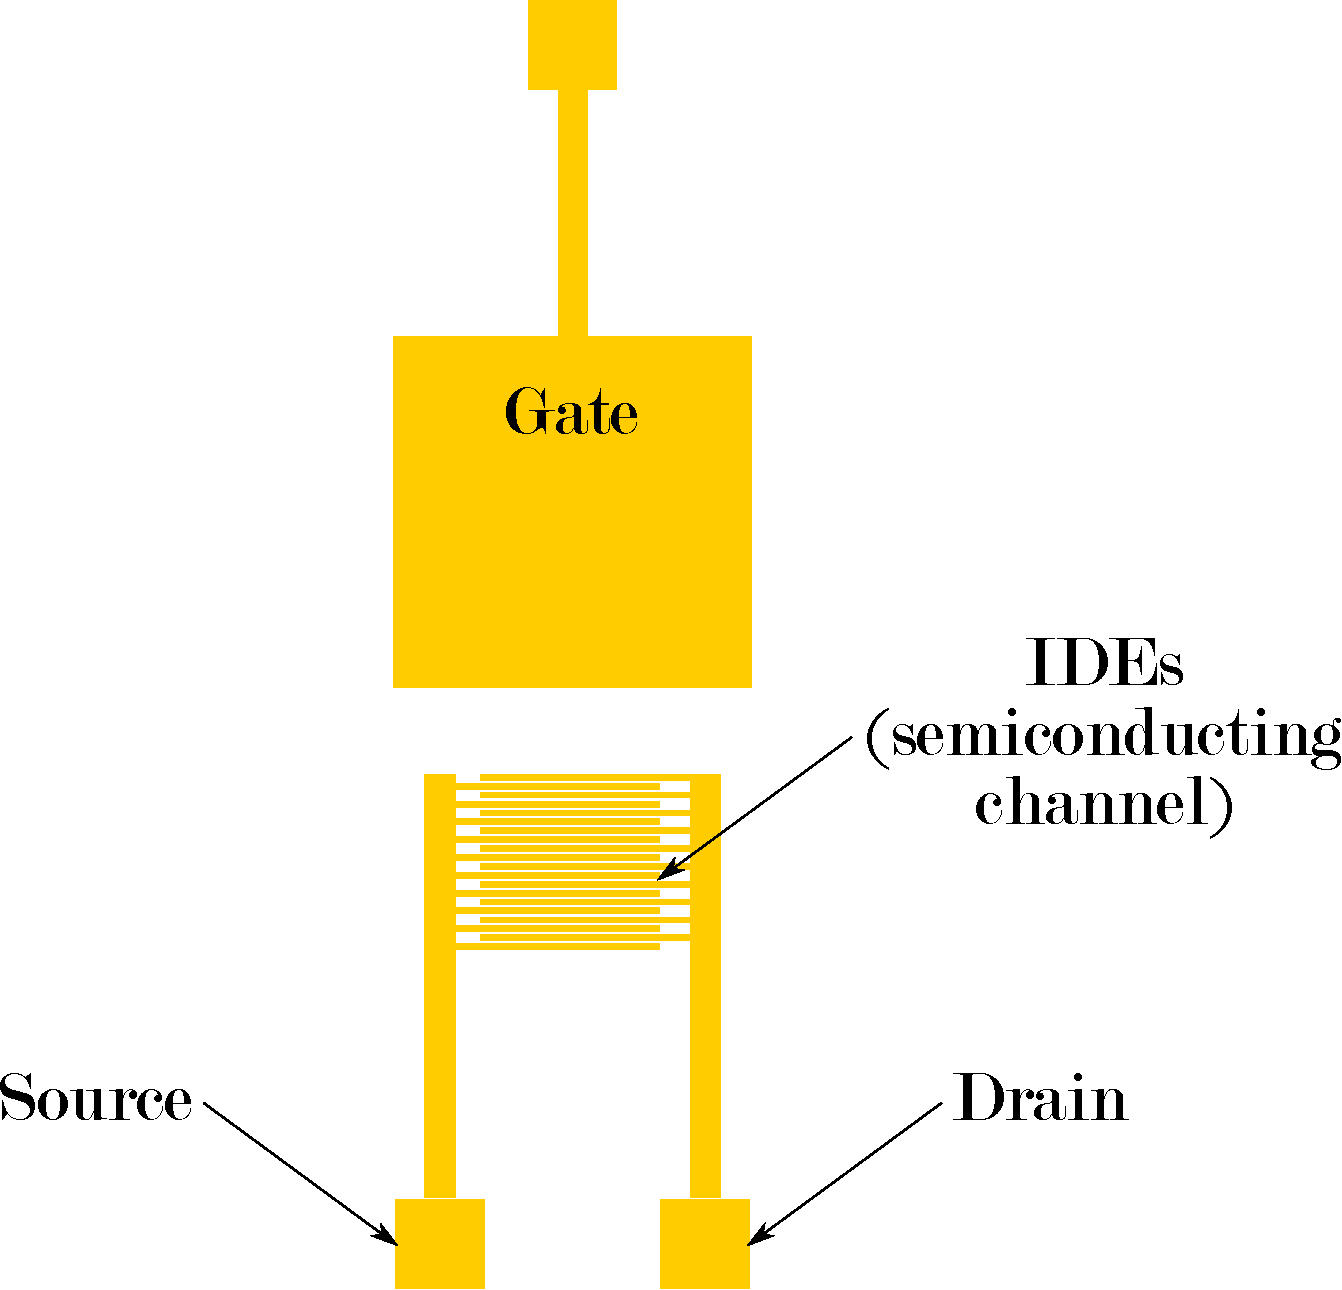
\includegraphics[width=0.3\textwidth]{figures/chapter3/EGFET/standardEGFET_scheme.pdf}
    \quad
    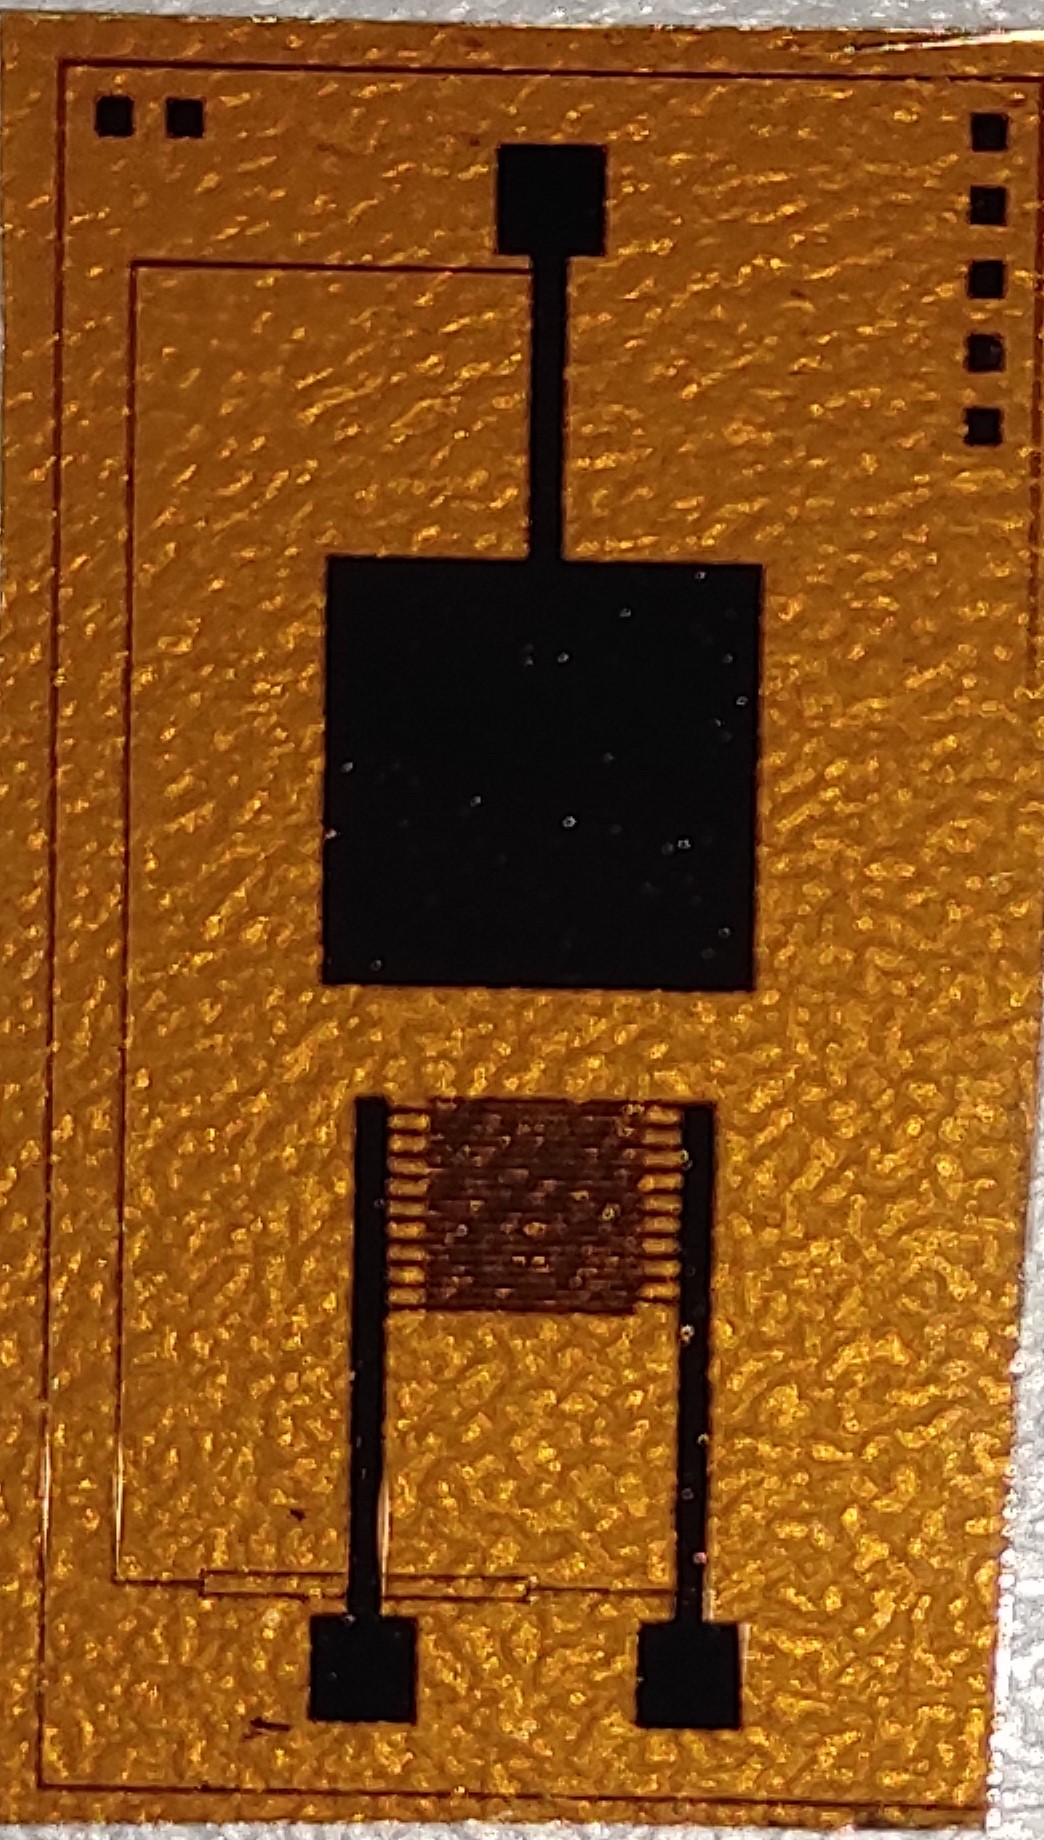
\includegraphics[width=0.16\textwidth]{figures/chapter3/EGFET/standardEGFET.jpg}
    \caption{The geometry of the standard EG-FET has been previously optimized by \citet{joshiUnderstanding2018}. The square gate has a side length of \SI{5.7}{\mm}, while the IDEs have a length of \SI{3}{\mm} and a height of \SI{100}{\um}. The channel length is \SI{50}{\um}, and due to the interdigitated design, the channel width amounts to \SI{57}{\mm}. The distance between the channel and gate is set to \SI{1.5}{\mm}.}
    \label{fig:standardEGFET}
\end{figure}

The standard EG-CNTFET geometry in Figure \ref{fig:standardEGFET} was based on the studies of \citet{joshiUnderstanding2018}, who evaluated different ratios between the gate area and the channel area; it was found that best performance was achieved by the configuration where the gate area was four times larger than the channel area. The IDEs are \SI{3}{\mm} long and \SI{100}{\um} high, with a channel width that amounts to \SI{57}{\mm}; this configuration results in a large $\frac{W}{L}$ ratio, which is linked to a high transconductance, as indicated in Equation \eqref{eq:transconductance}. A big transconductance leads to an increased sensitivity of the device to small variations in gate potential, thus making it more responsive to changes in the applied voltage. Finally, a planar \SI{5.7}{\mm} $\times$ \SI{5.7}{\mm} gate electrode was employed.

The deposition of SWCNTs onto the devices was carried out following the protocol previously optimized by \citet{shkodraOptimization2023}, as described in Section \ref{sec:cntDeposition}. Following this protocol, 60 layers of SWCNTs were deposited, leading to a post-deposition \rds{} between \SIrange{1}{10}{\kohm}; in fact, it was observed by \citet{petrelliMethod2023} that this range is where the performance of this type of device is optimal. In addition, this step provided an initial skimming of the manufactured devices, in order to reduce device-to-device variability that could be detrimental to subsequent steps.

The devices that passed this screening were subjected to electrical characterization, by collecting transfer characteristics, according to the protocol given in Section \ref{sec:characterization}. First the raw transfer curves were observed, without any processing (Figure \ref{fig:transferNoMem}), after which the variation of the ON current (\ion{}) was evaluated as a function of time (Figure \ref{fig:NormNoMem}). Normalization was performed by taking the \ion{} value at \vgs{}=\SI{-0.8}{\V} for each cycle and dividing it by the \ion{} of the first recorded transfer curve during that measurement sequence. This approach is useful to standardize the current variations across different devices, allowing a fair comparison of their performance. While the measured current was always considered, normalization helped in further mitigating the influence of device-to-device variation, thus facilitating the comparison among different devices, without interference from fabrication inconsistencies.
The observation of transfer characteristics shows that the \ids{} decreases progressively after each measurement cycle, although this trend is more clearly seen in the normalized \ion{} over time. This decrease indicates that there is a level of degradation of CNTs and that something occurs during their use that alters their functionality. This effect is not particularly relevant during the 60-minute measurement, though it can become a problem for longer measurements, as in the case of EG-CNTFET used as a transducer for a sensor. Calibration measurements, in fact, can take several hours; during this time there is a risk that the measured current will continuously decrease until it reaches \SI{0}{\uA}, making the measurements unreliable.

\begin{figure}
    \centering
    \subfloat[Transfer characteristics]{%
        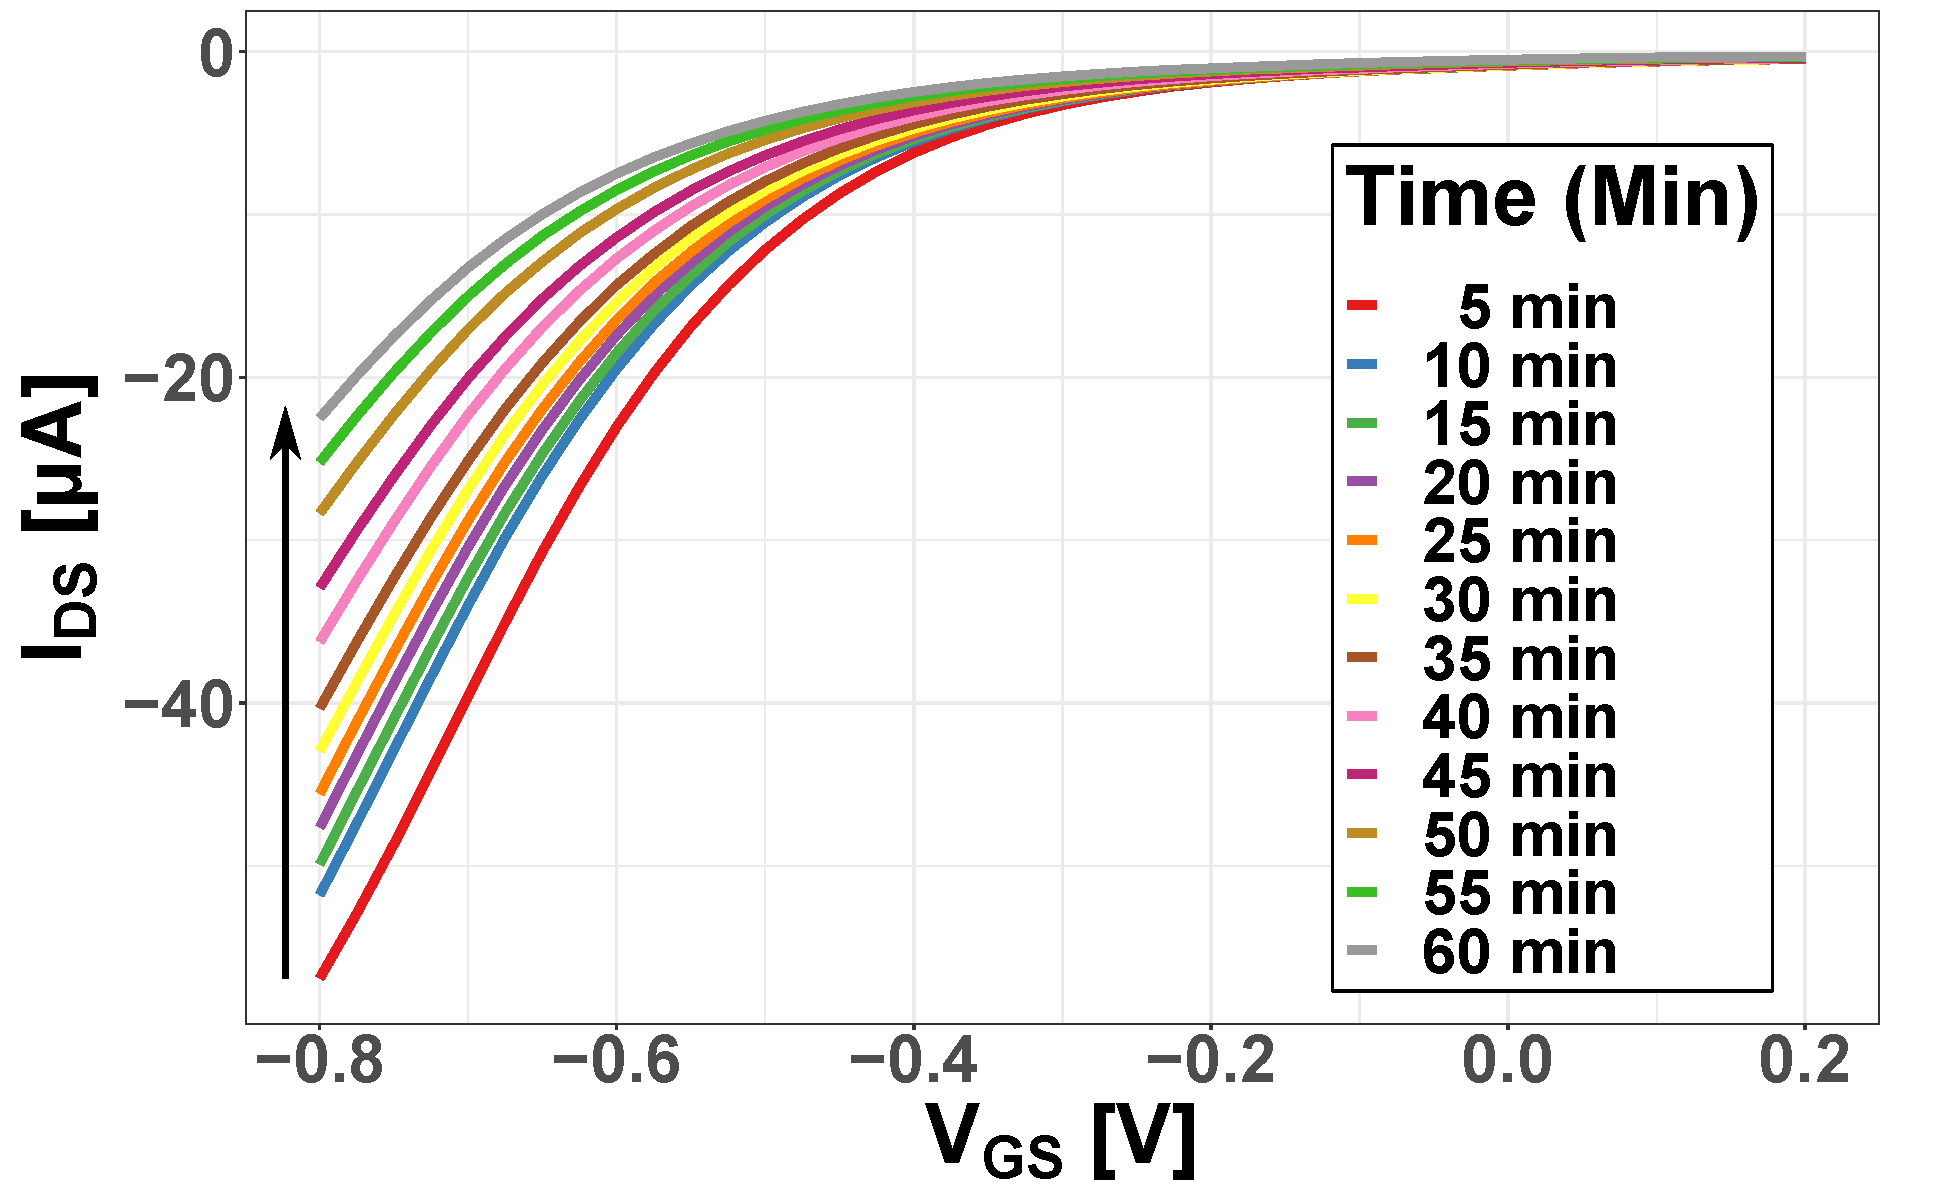
\includegraphics[width=0.45\textwidth]{figures/chapter3/EGFET/transferNoMem.pdf}%
        \label{fig:transferNoMem}
    }
    \quad
    \subfloat[Normalized \ion{}]{%
        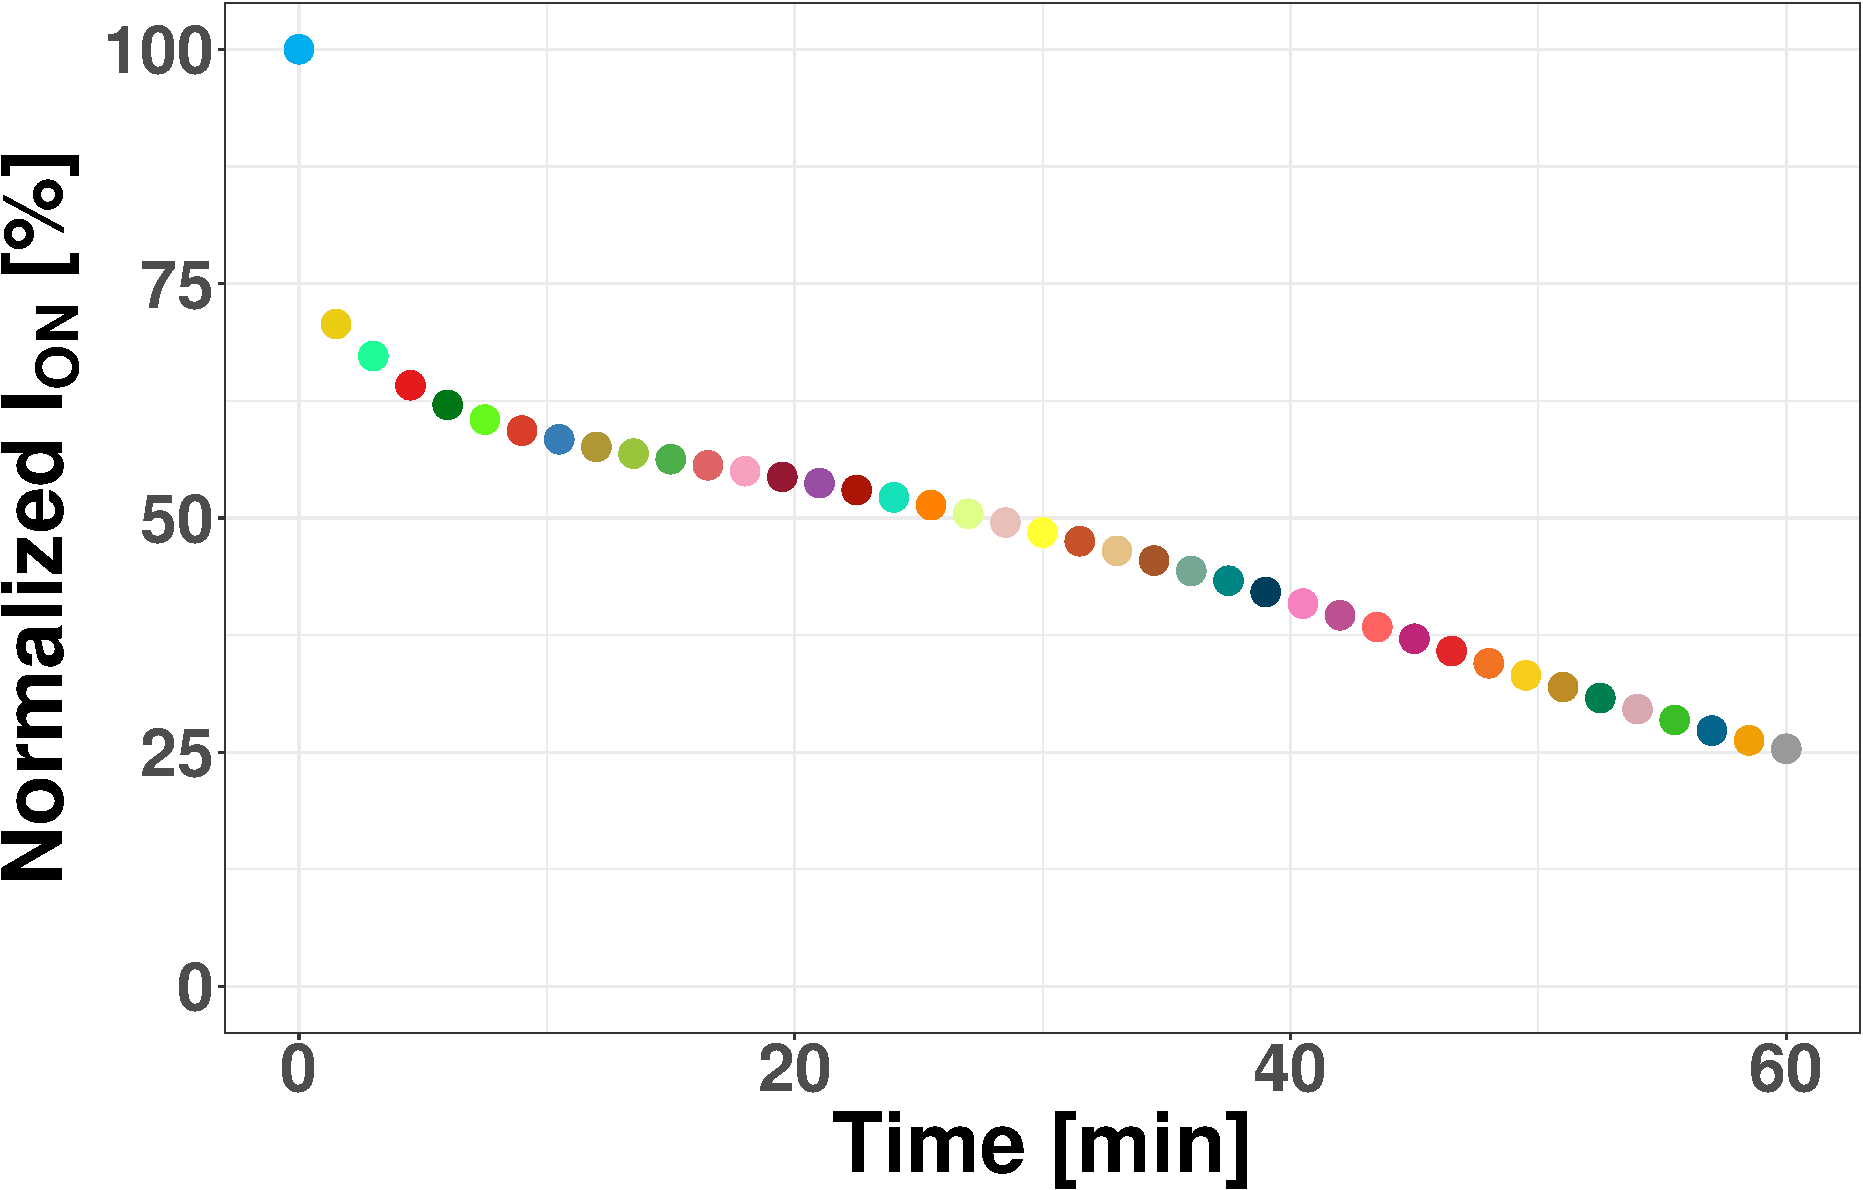
\includegraphics[width=0.45\textwidth]{figures/chapter3/EGFET/NormNoMem.pdf}%
        \label{fig:NormNoMem}
    }
    \caption{Electrical characterization of a standard EG-CNTFET device. 
    (a) The consecutive transfer curves collected over the span of \SI{60}{\min} show that the current decreases prograssively after each measurement, as indicated by the arrow.
    (b) The normalized \ion{} for the same device better highlights the phenomenon of decreasing current, indicating device instability. It is important to note that this instability may compromise the reliability of the platform when used for longer times, as it happens for sensing applications.}
    \label{fig:noMem}
\end{figure}

\begin{figure}
    \centering
    \subfloat[\igs{} and \ids{}]{%
        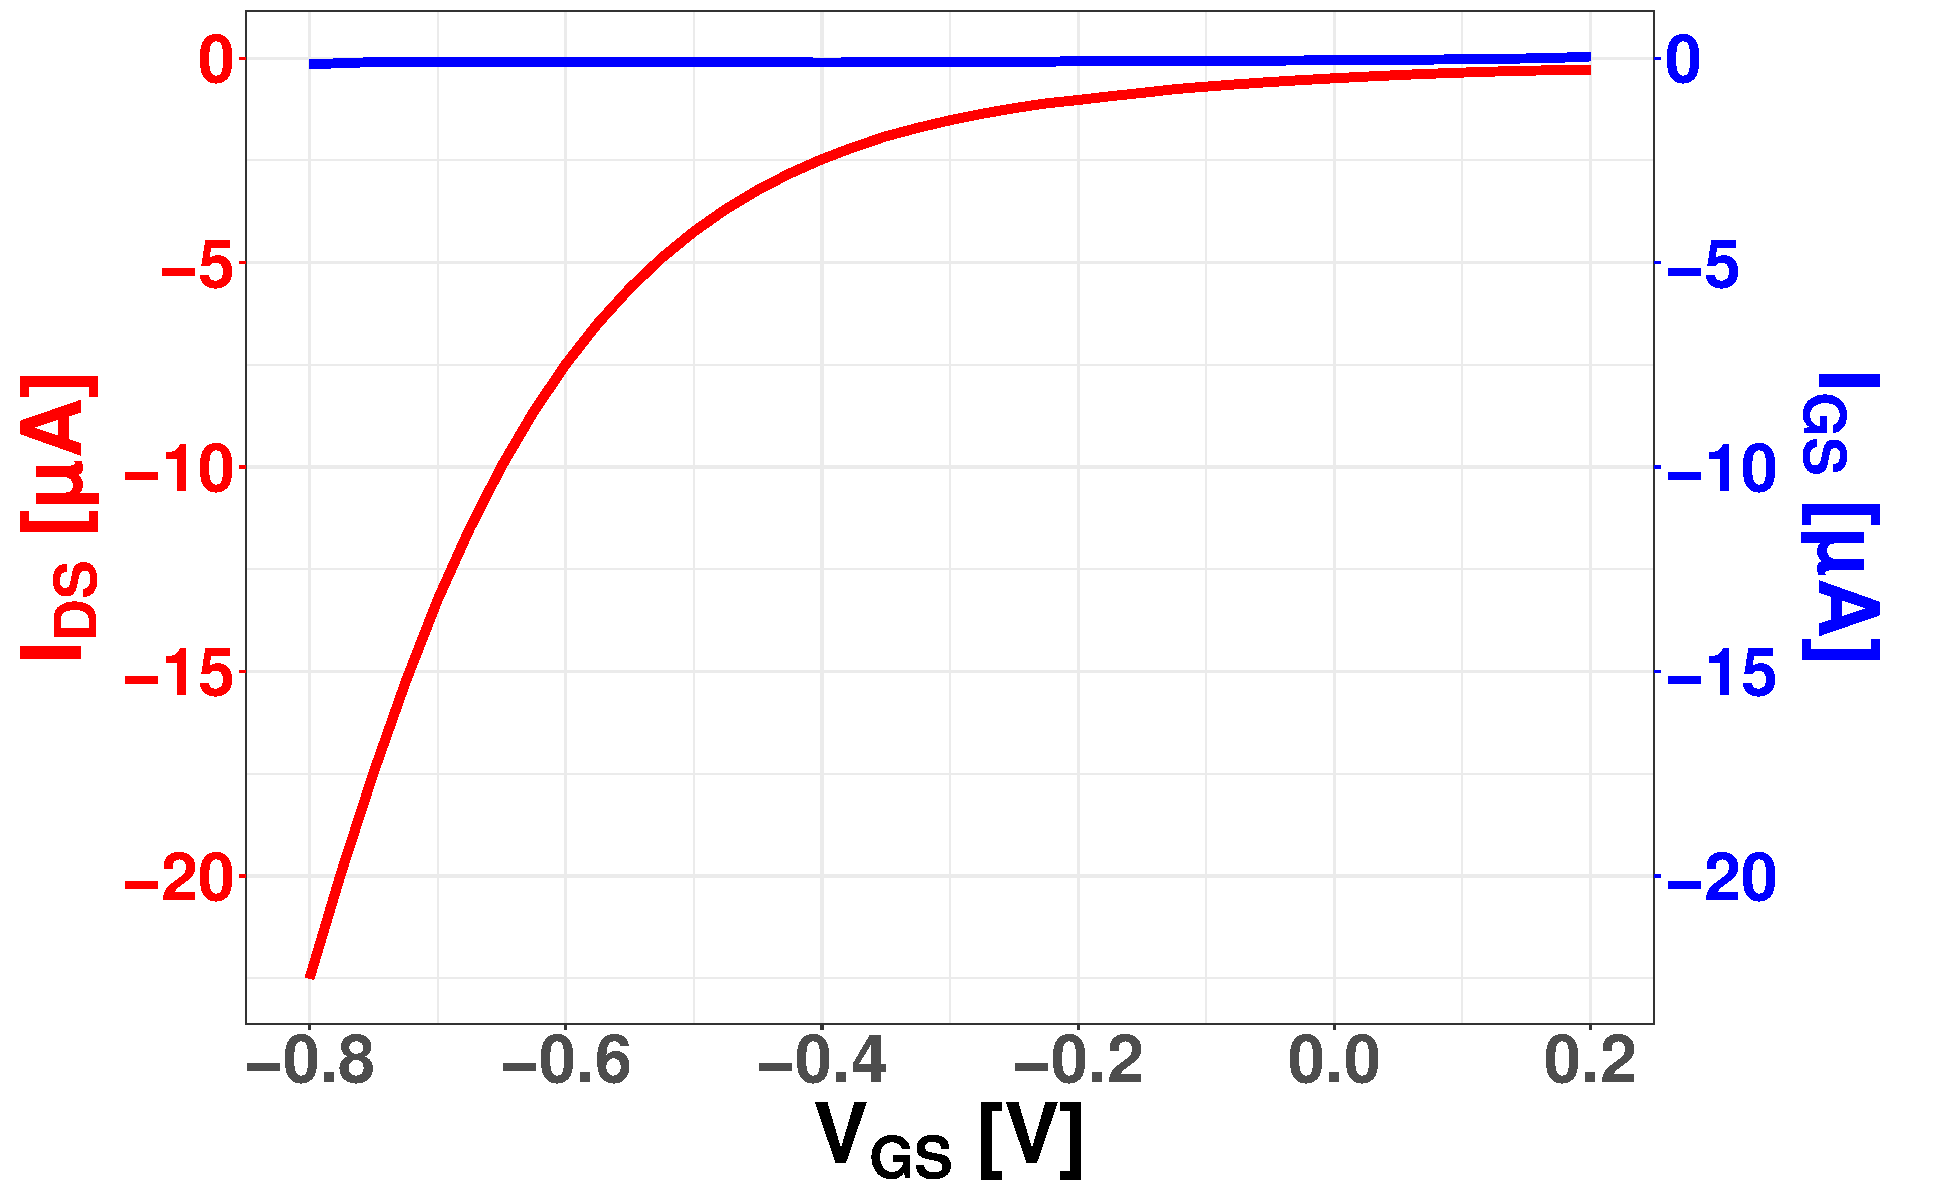
\includegraphics[width=0.45\textwidth]{figures/chapter3/EGFET/IdIgNoMem.pdf}%
        \label{fig:IdIgNoMem}
    }
    \quad
    \subfloat[Hysteresis]{%
        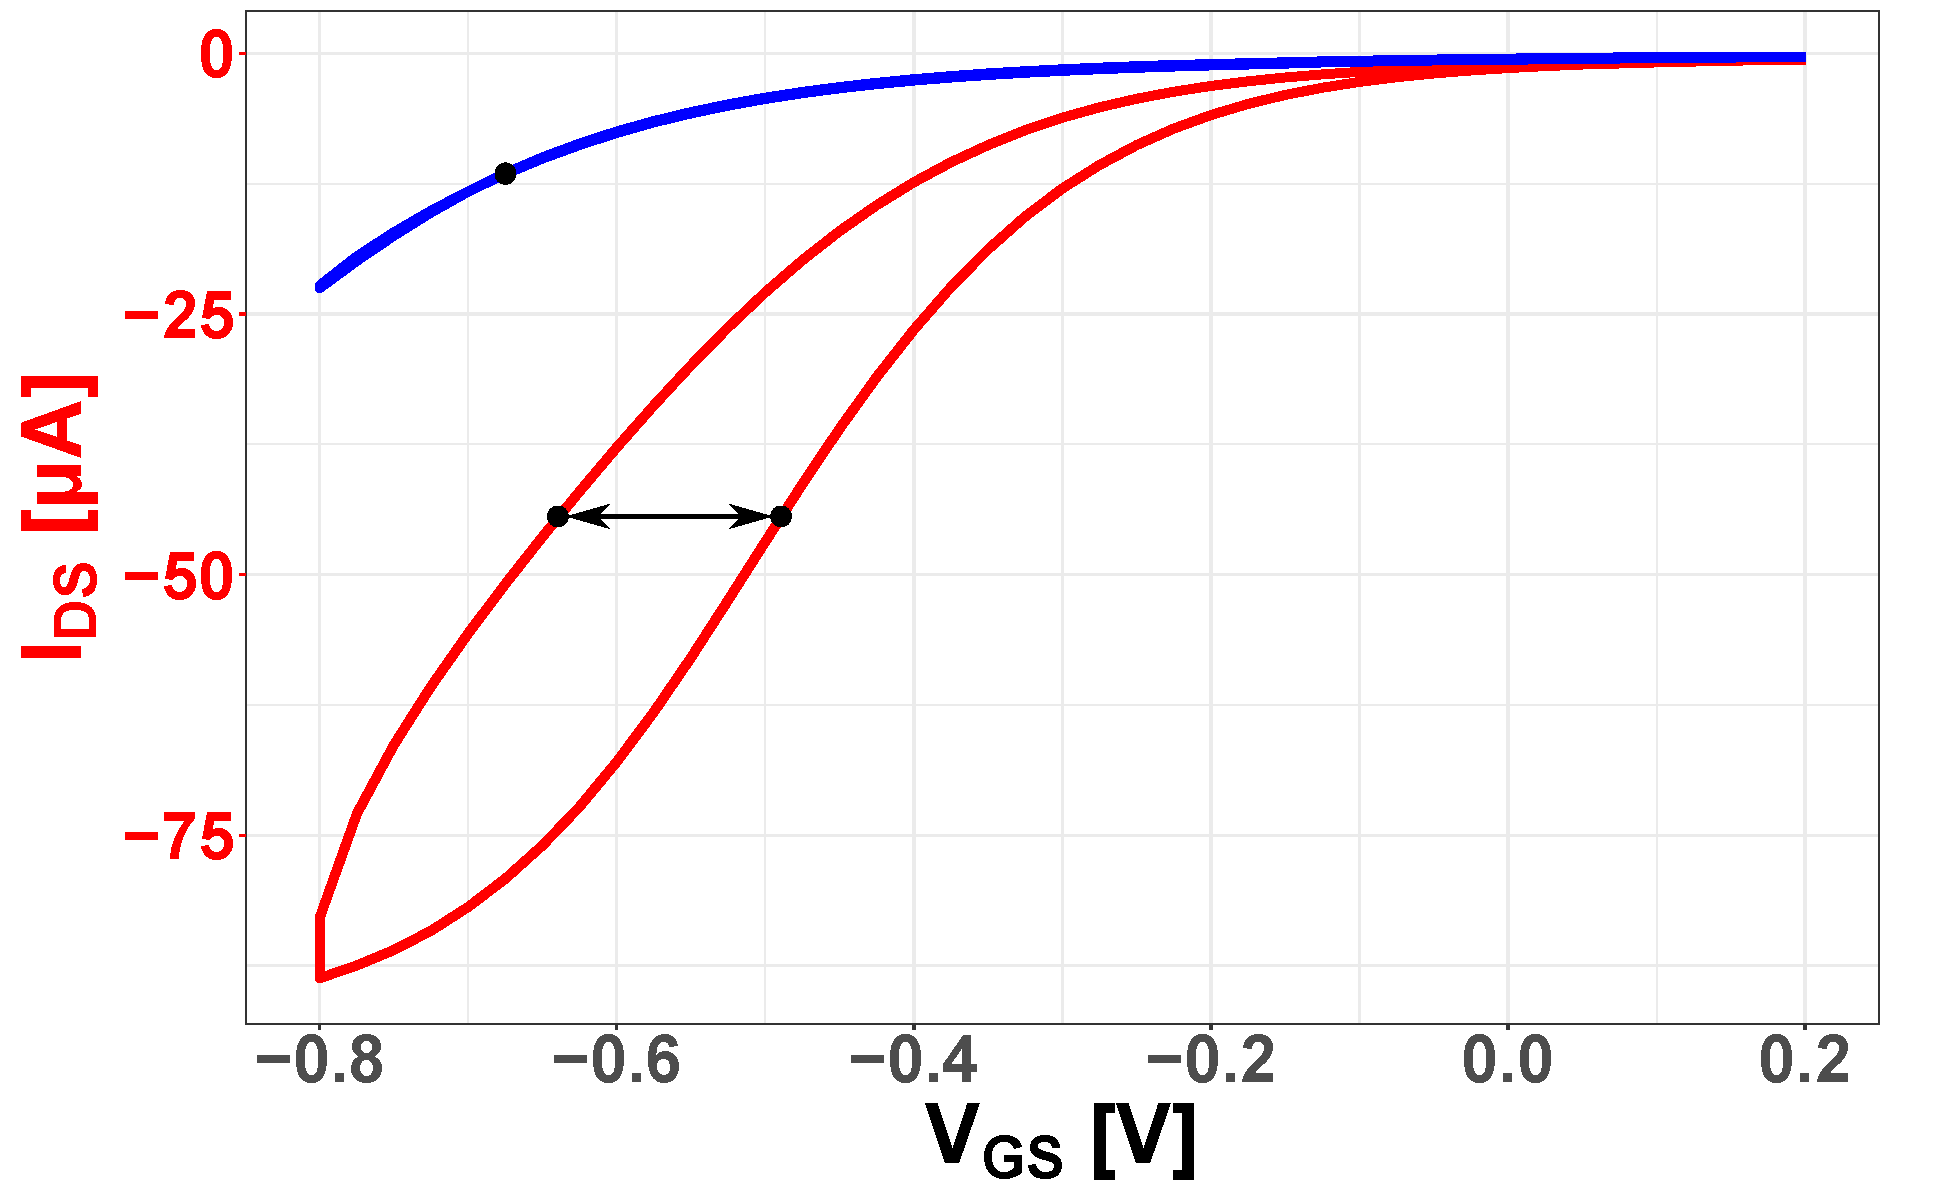
\includegraphics[width=0.45\textwidth]{figures/chapter3/EGFET/hysNoMem.pdf}%
        \label{fig:hysNoMem}
    }
    \caption{Electrical characterization of the EG-CNTFET devices. 
    (a) Gate current (\igs{}) and drain current (\ids{}): \igs{} is several orders of magnitude lower than \ids{}, indicating low gate leakage. This suggests efficient gate control, reduced power dissipation, and minimized unintended electrochemical reactions at the gate interface, all of which contribute to improved device performance and longevity. 
    (b) Hysteresis decreases greatly from the first (red curve) to the last transfer curve (blue curve), indicating a more stable operation over time.}
    \label{fig:parameters_noMem}
\end{figure}

Figure \ref{fig:IdIgNoMem} shows \ids{} and \igs{} on the same plot: \igs{} is orders of magnitude lower than \ids{}, indicating minimal gate leakage, which is crucial for efficient transistor functioning. Indeed, gate leakage is a phenomenon that occurs when a current flows between the gate and the channel, exiting the designated source-drain path, leading to increased power dissipation, and reduced device efficiency and stability.

Another parameter to consider in device performance is hysteresis, which is defined as \vv{the difference of the voltages that should be applied to the gate in forward and backwards sweeps to get the drain current equal to the average of maximum and minimum drain current, \ie{} ($\frac{I_{\text{D,max}} + I_{\text{D,min}}}{2}$)} \citep{joshiUnderstanding2018}. Several factors contribute to hysteresis, including adsorbed water and oxygen molecules on the CNT surface, and surface traps that capture induced charges \citep{joshiUnderstanding2018,zaumseilSemiconducting2019}. Hysteresis is an important parameter to evaluate, as it can significantly impact device performance: indeed it can affect mobility, threshold voltage, on/off ratio, and sub-threshold slope, potentially causing signal drift and negatively impacting reliability \citep{joshiUnderstanding2018,noyceElectronic2019}.

As shown in Figure \ref{fig:hysNoMem}, hysteresis in the devices herein presented significantly decreases over time, indicating that device performance improves over time. However, it is important to observe that this reduction in hysteresis is concomitant with a decrease in \ids{} that cannot be overlooked.

\note{\AT{VOGLIO INSERIRE QUESTA FRASE AD UN CERTO PUNTO} This trade-off must be carefully considered when assessing long-term device performance and reliability.}

\begin{figure}[hb]
    \centering
    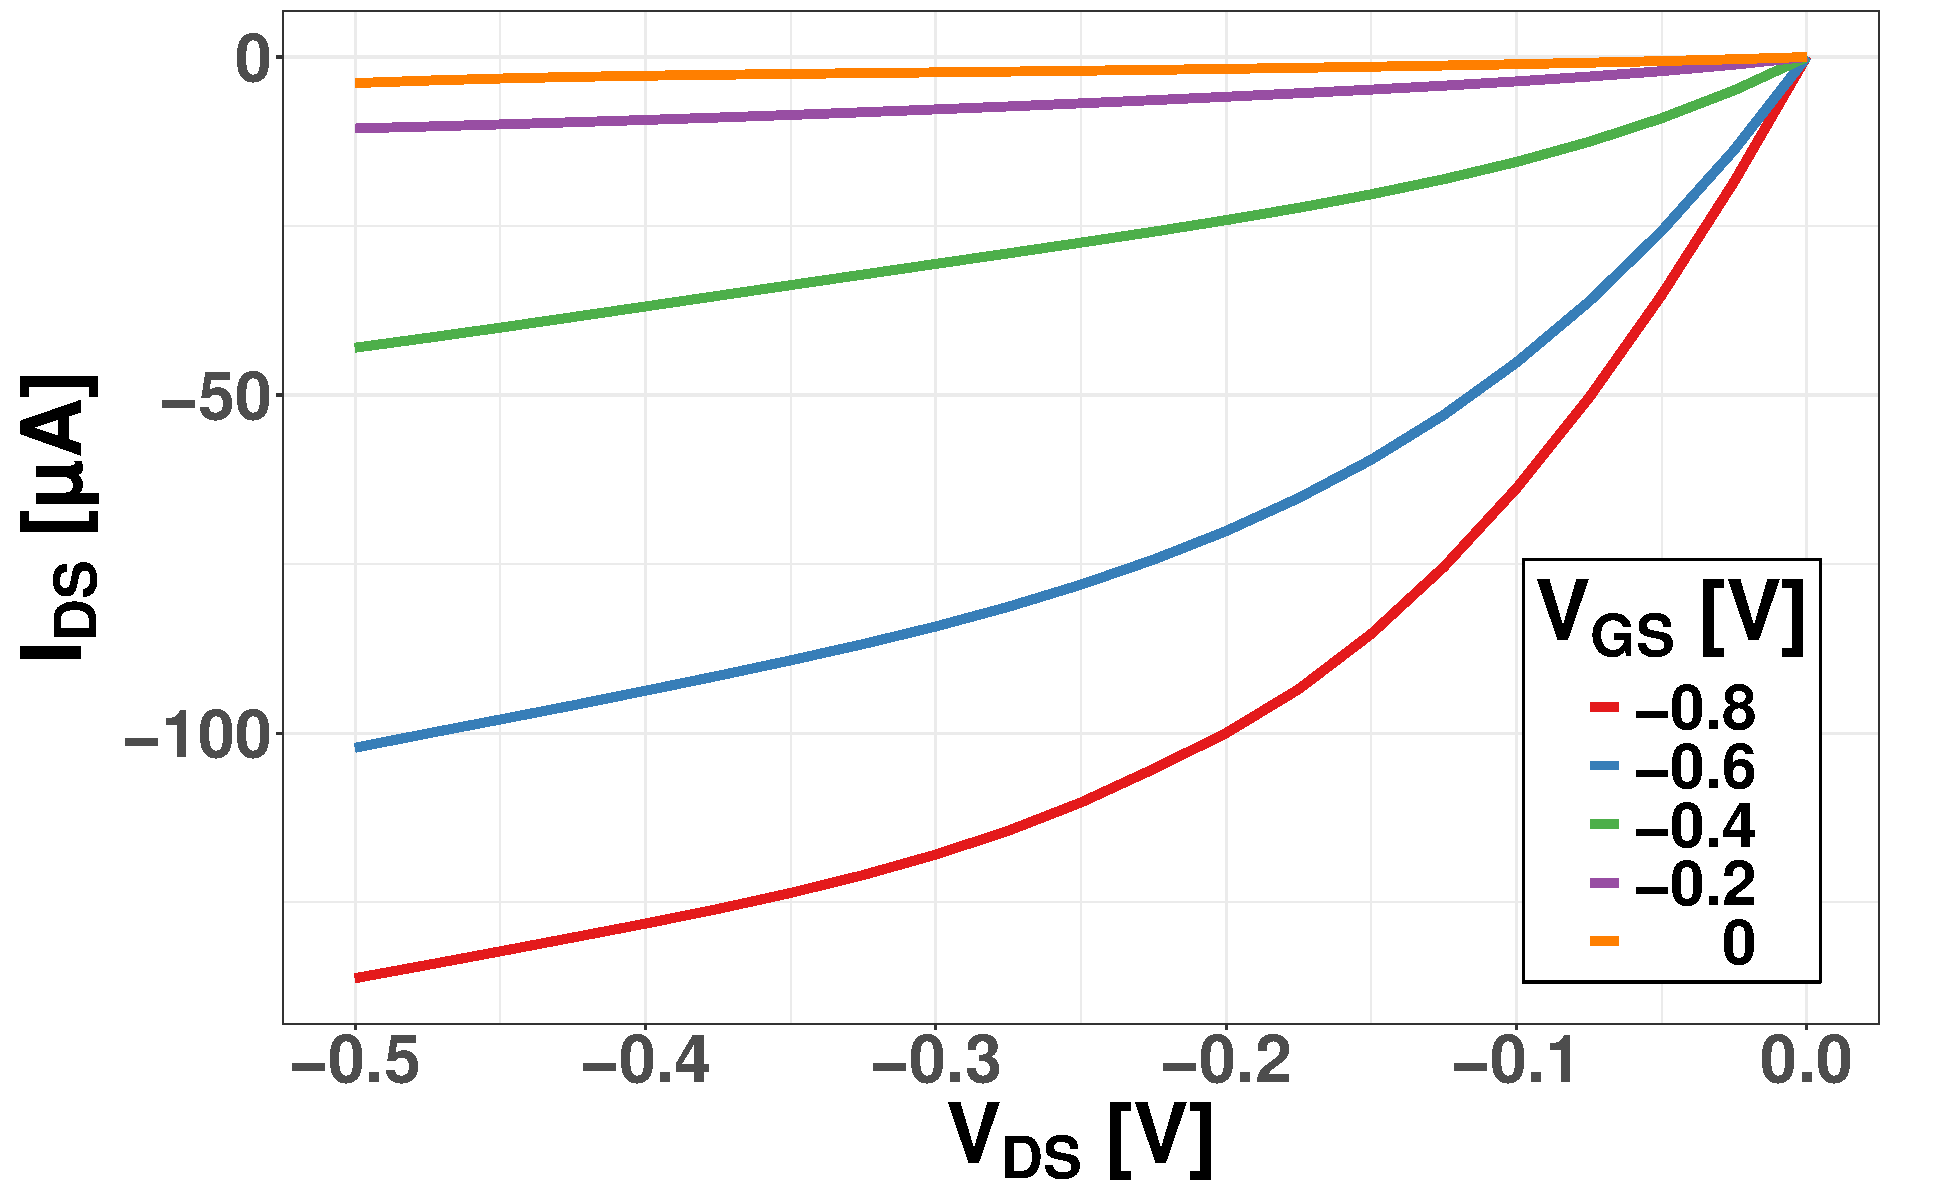
\includegraphics[width=0.45\textwidth]{figures/chapter3/EGFET/outputNoMem.pdf}
    \caption{Electrical characterization of a standard EG-CNTFET device. Output characteristics: the device operates in the linear regime for all \vds{}, although it approaches saturation at \SI{-0.6}{\V} and \SI{-0.8}{\V}. This is supported by the approximately linear trend, which precisely suggests operation in the ohmic region, indicating low contact resistance and efficient charge injection. The well-defined current modulation across different \vgs{} values demonstrates effective gate control, which is essential for stable transistor operation and reliable switching behavior.}
    \label{fig:outputNoMem}
\end{figure}

After the transfer curves, output characteristics were plotted and evaluated (Figure \ref{fig:outputNoMem}): output characteristics describe the relationship between \ids{} and \vds{} for different \vgs{}. By collecting output characteristics, it is possible to further assess device performance by extrapolating other parameters; in particular, observing these curves allowes to evaluate whether a device operates in linear or saturation regime. Indeed, from the curves displayed in Figure \ref{fig:outputNoMem}, it is possible to gather that the devices approach saturation but do not fully reach it. In fact, in a well-saturated regime, \ids{} would become relatively constant with increasing \vds{}; the incomplete saturation seen in these devices suggests that there may be residual channel conduction even at high \vds{}, due to factors such as inefficient carrier pinch-off, contact resistance, or electrostatic limitations of the electrolyte gating mechanism.

\subsection{Membrane encapsulation}
\label{sec:membrane_encapsulation}

With a baseline established, it is evident that the devices are not stable over time, as demonstrated by the decreasing current over time. The objective of this project was to develop an inexpensive approach to improve device stability while also achieving faster stabilization. To tackle this issue, a lipophilic membrane was deposited on the CNTs of the channel to protect them from environmental exposure. Indeed, CNTs degrade upon contact with the oxygen in the air and with the water molecules of the electrolyte, causing an alteration in device performance. Great care must be therefore given to these devices, to the point that they must be stored in a protected environment, \ie{} a nitrogen-filled glovebox, to prevent damages to the nanotubes in the time prior to the measurements. Additionally, during the measurements, CNTs are exposed to the ions contained in the electrolyte, which could react with the functional groups on the nanotubes and thus further contribute to the worsening performance.

The first step in this approach was optimizing the membrane deposition process itself, \ie{} the volume to be dropcast and the resulting membrane thickness. Initially, \SI{10}{\ul} of the membrane were dropcasted onto the CNT channel in a one-step deposition. This proved insufficient in providing consistent protection: 50\% of devices reached higher stability, while the other half still exhibited worsening behaviour during measurements, indicating that the CNTs were still suffering the consequences of air and electrolyte exposure ($N = 12$). Given this variability, an alternative deposition strategy needed to be developed to ensure a more reliable coverage.
It was found that a two-step dropcasting process, \ie{} first depositing \SI{8}{\ul} and following with an additional \SI{7}{\ul}, resulted in effective CNT coverage while still allowing current to flow.

\begin{figure}
    \centering
    \subfloat[]{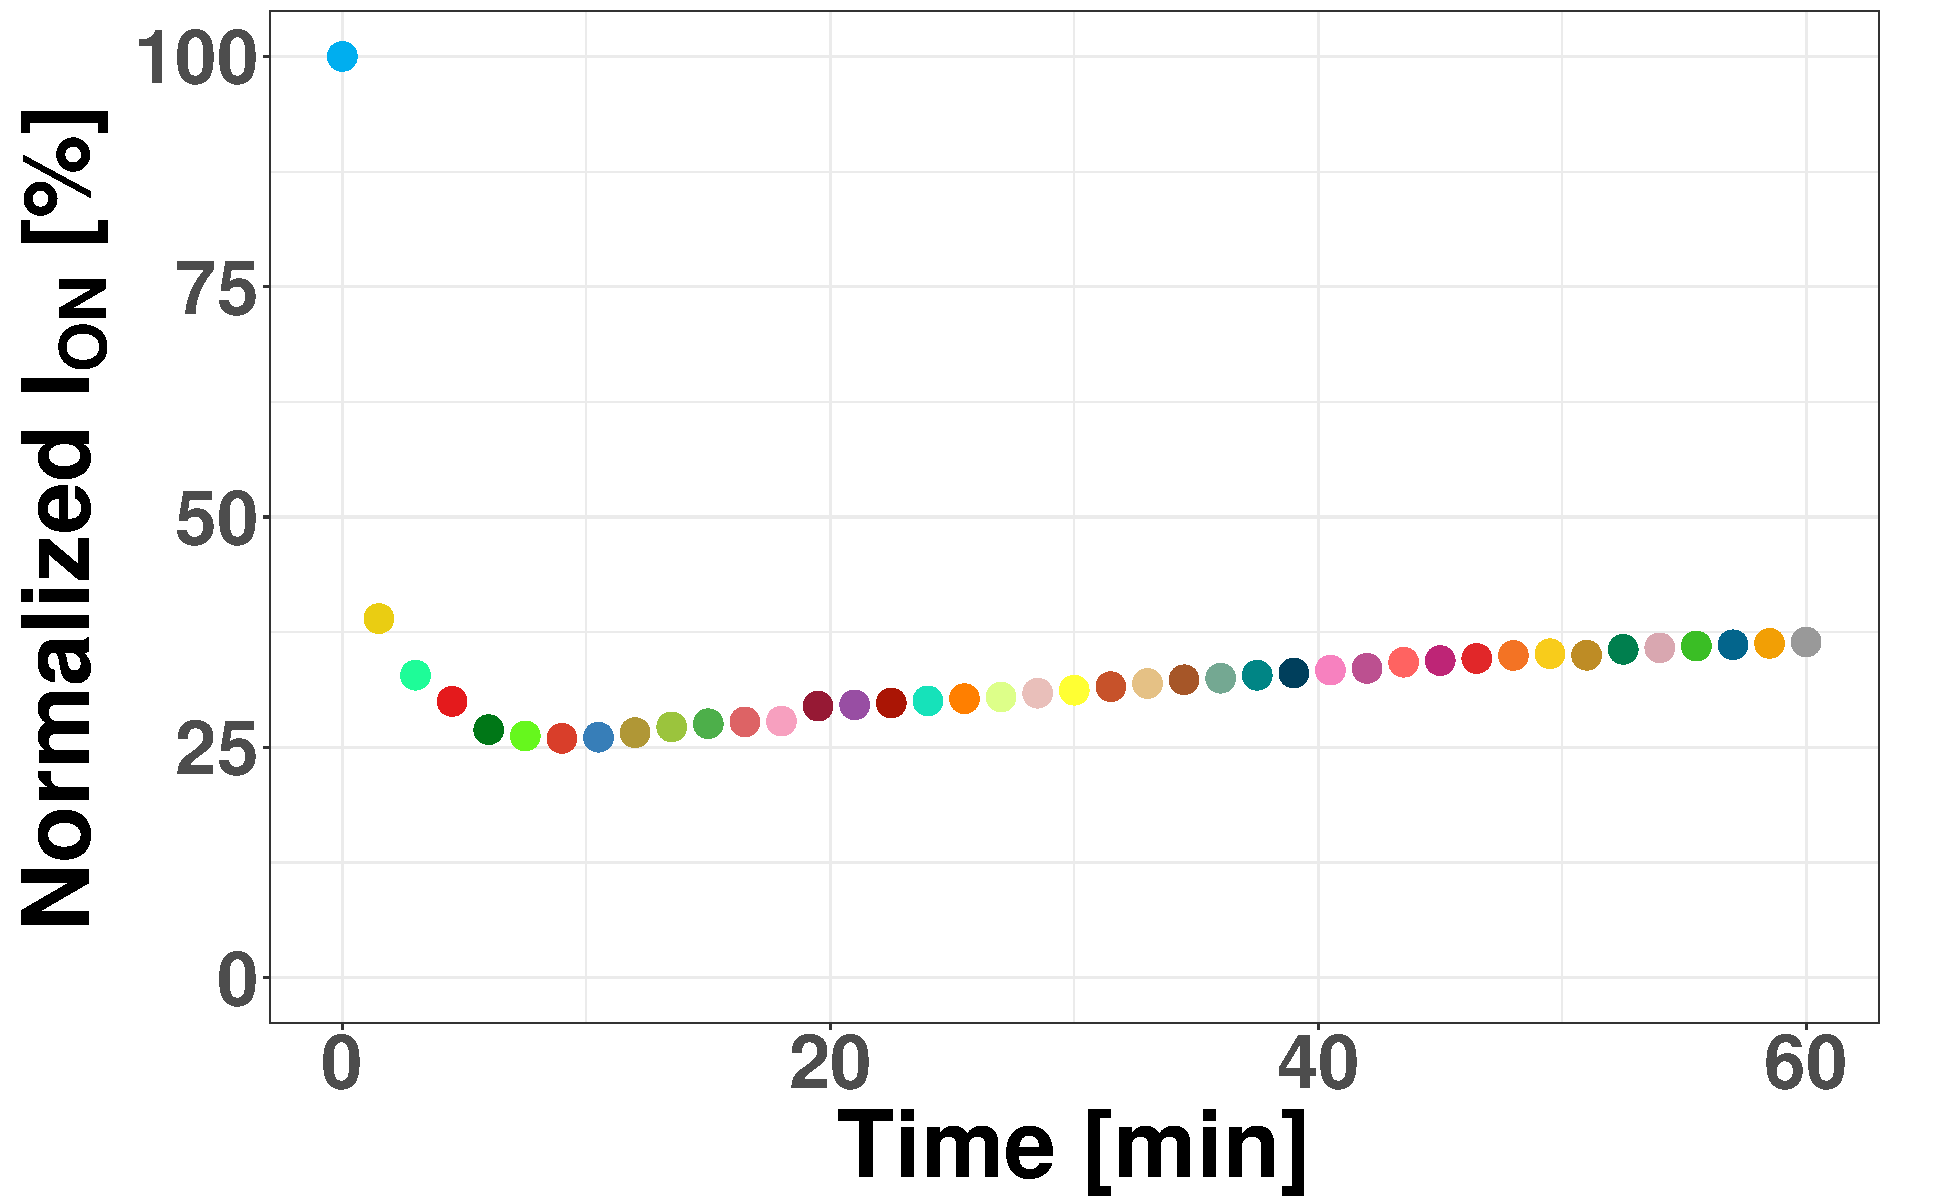
\includegraphics[width = 0.45\textwidth]{figures/chapter3/EGFET/norm_good.pdf}}
    \subfloat[]{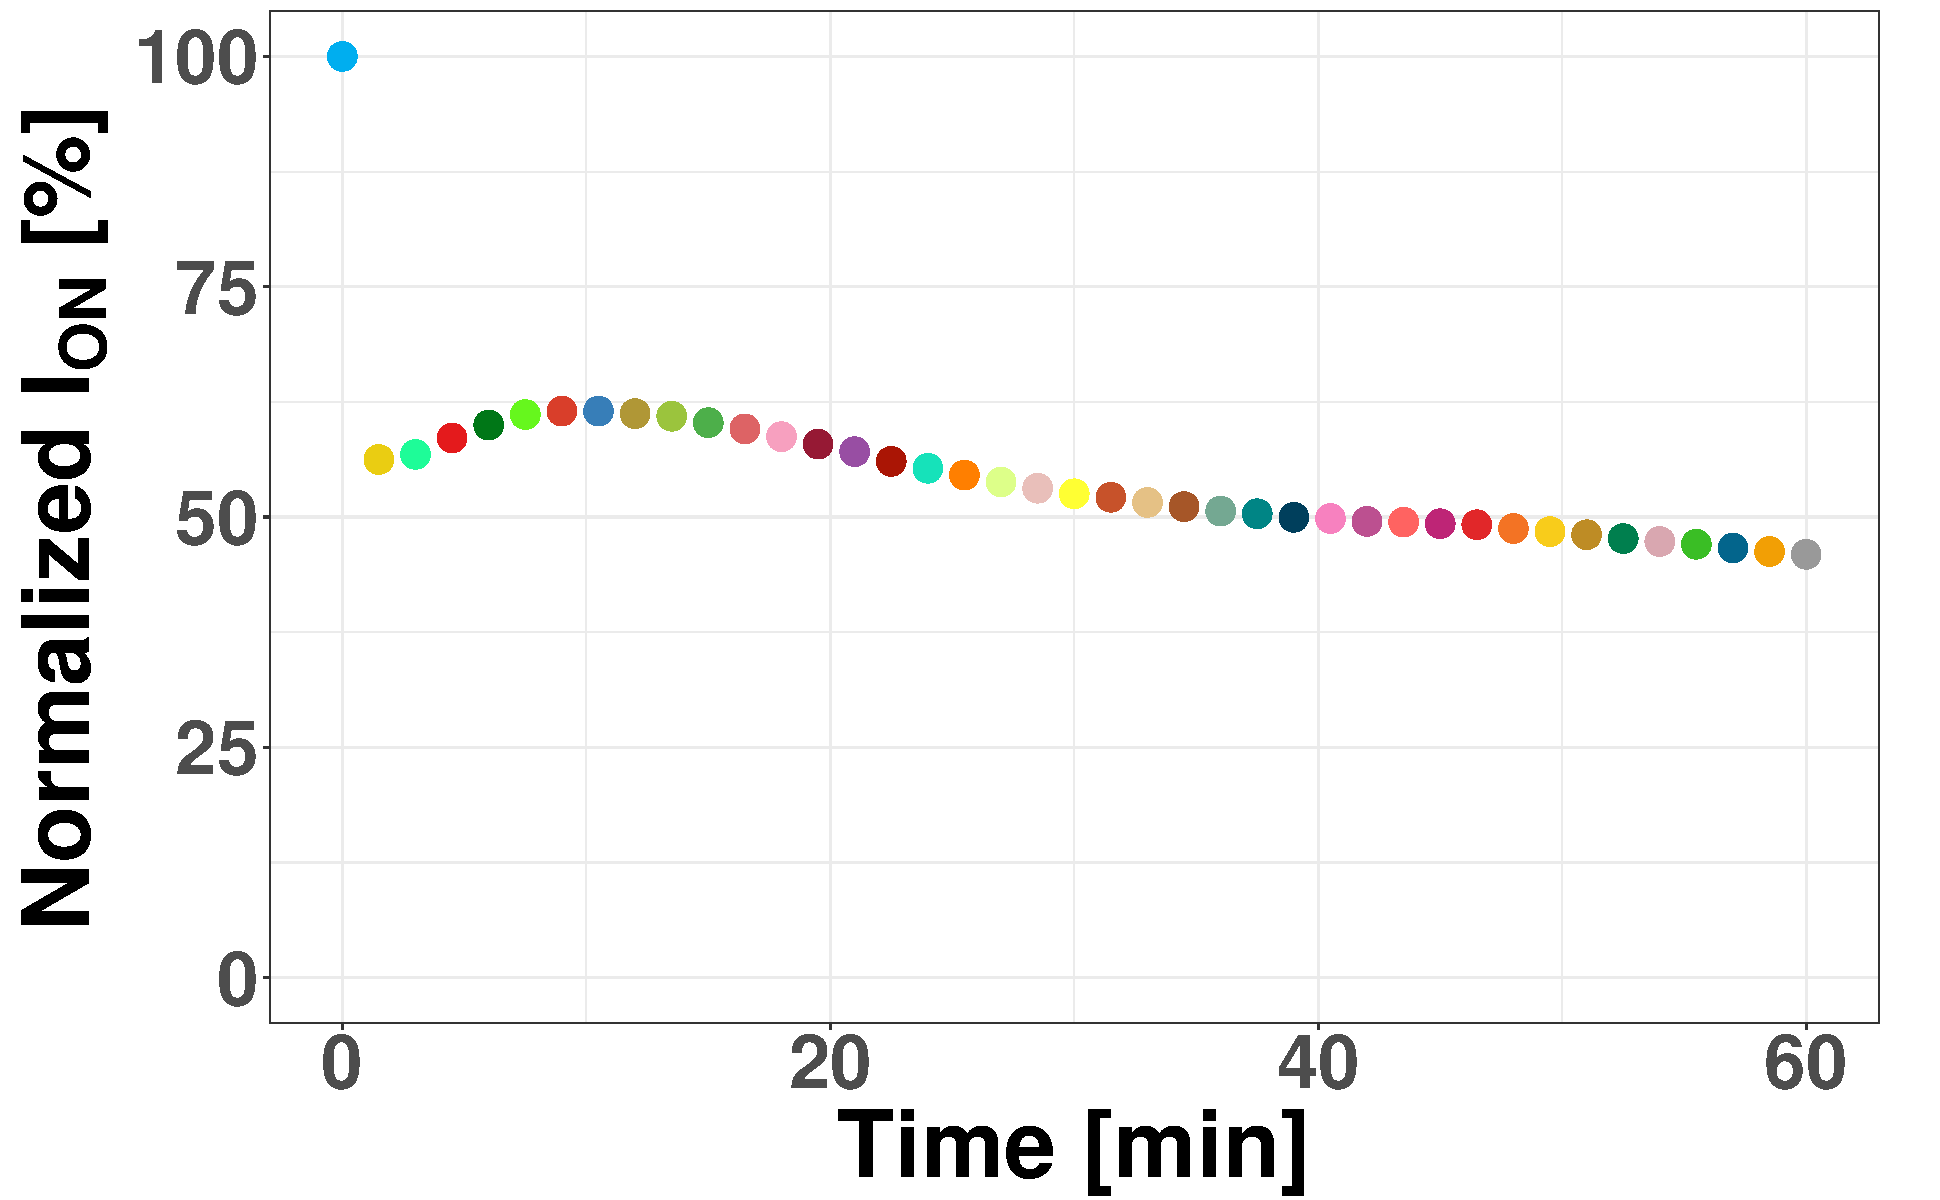
\includegraphics[width = 0.45\textwidth]{figures/chapter3/EGFET/norm_bad.pdf}}
    \caption{\AT{I need the caption to a figure for a scientific paper: the figure contains the comparison of two images showing the normalized \ids{} of two standard EG-FETs with 10\textmu{}l of lipophilic membrane dropcasted on the channel. The results are mixed, with some devices stabilizing, aka. the current increases over time, while other devices remain unstable, as if they had no membrane, meaning that the CNTs are still vulnerable to the environment.} \note{Comparison of the normalized \ids{} of two standard EG-FETs with \SI{10}{\micro\liter} of lipophilic membrane dropcasted on the channel. The results show mixed behavior: some devices stabilize over time, as indicated by the increasing current, while others remain unstable, behaving as if they had no membrane. This suggests that in certain cases, the CNTs remain vulnerable to environmental influences.}}
    \label{fig:membrane10ul}
\end{figure}

\begin{figure}
    \centering
    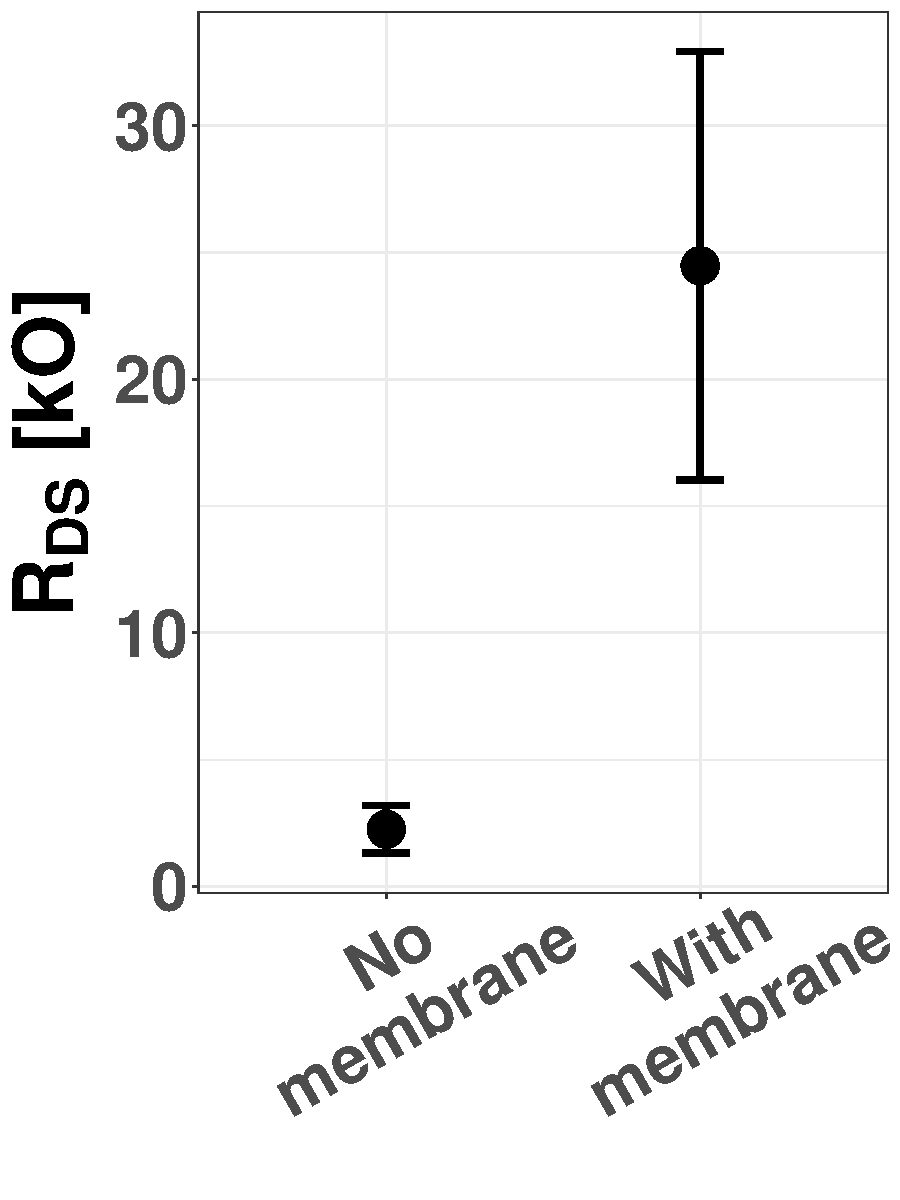
\includegraphics[width = 0.3\textwidth]{figures/chapter3/EGFET/Rds_change.pdf}
    \caption{\AT{I need the caption to a figure for a scientific paper: this figure shows the variation in resistance between source and drain before and after the deposition of the lipophilic membrane. This value shows that before the membrane, the devices have a resistance of approximately \SI{2.5}{\kohm}, with very little variability among them (a selection of devices had already been done, exactly for the purpose of having the best performing platforms, while also reducing device-to-device variability). After membrane deposition, the resistance increases, and with it, the standard deviation, aka the variability among the devices.} \note{Variation in resistance between source and drain before and after the deposition of the lipophilic membrane. Before membrane deposition, the devices exhibit a resistance of approximately \SI{2.5}{\kohm}, with minimal variability among them, as a pre-selection process was carried out to ensure optimal performance and reduced device-to-device variation. After membrane deposition, the resistance increases, accompanied by a rise in standard deviation, indicating greater variability among the devices.}}
    \label{fig:rdsChange}
\end{figure}

\begin{figure}
    \centering
    \subfloat[Transfer characteristics]{%
        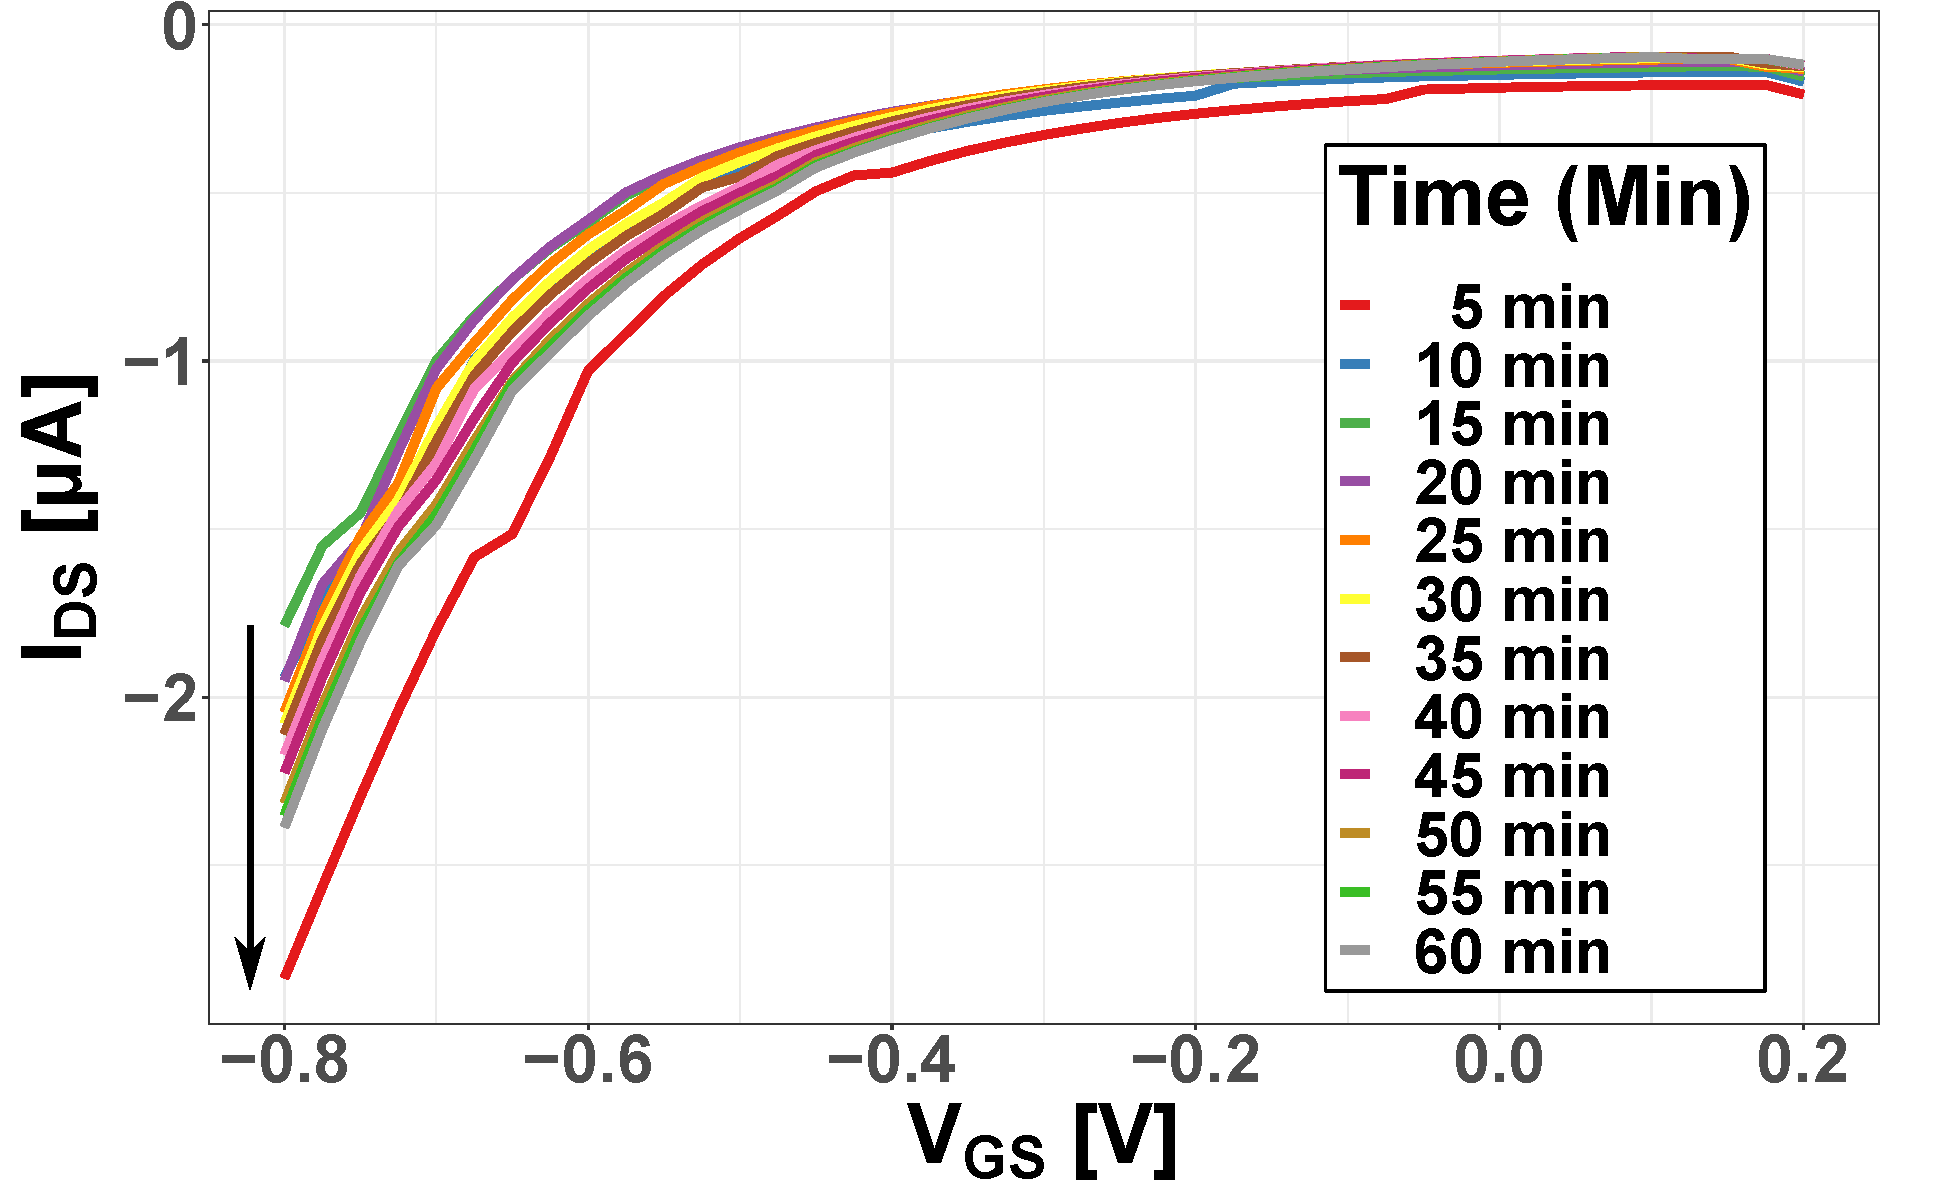
\includegraphics[width=0.45\textwidth]{figures/chapter3/EGFET/transferMem.pdf}%
        \label{fig:transferMem}
    }
    \quad
    \subfloat[Normalized \ion{}]{%
        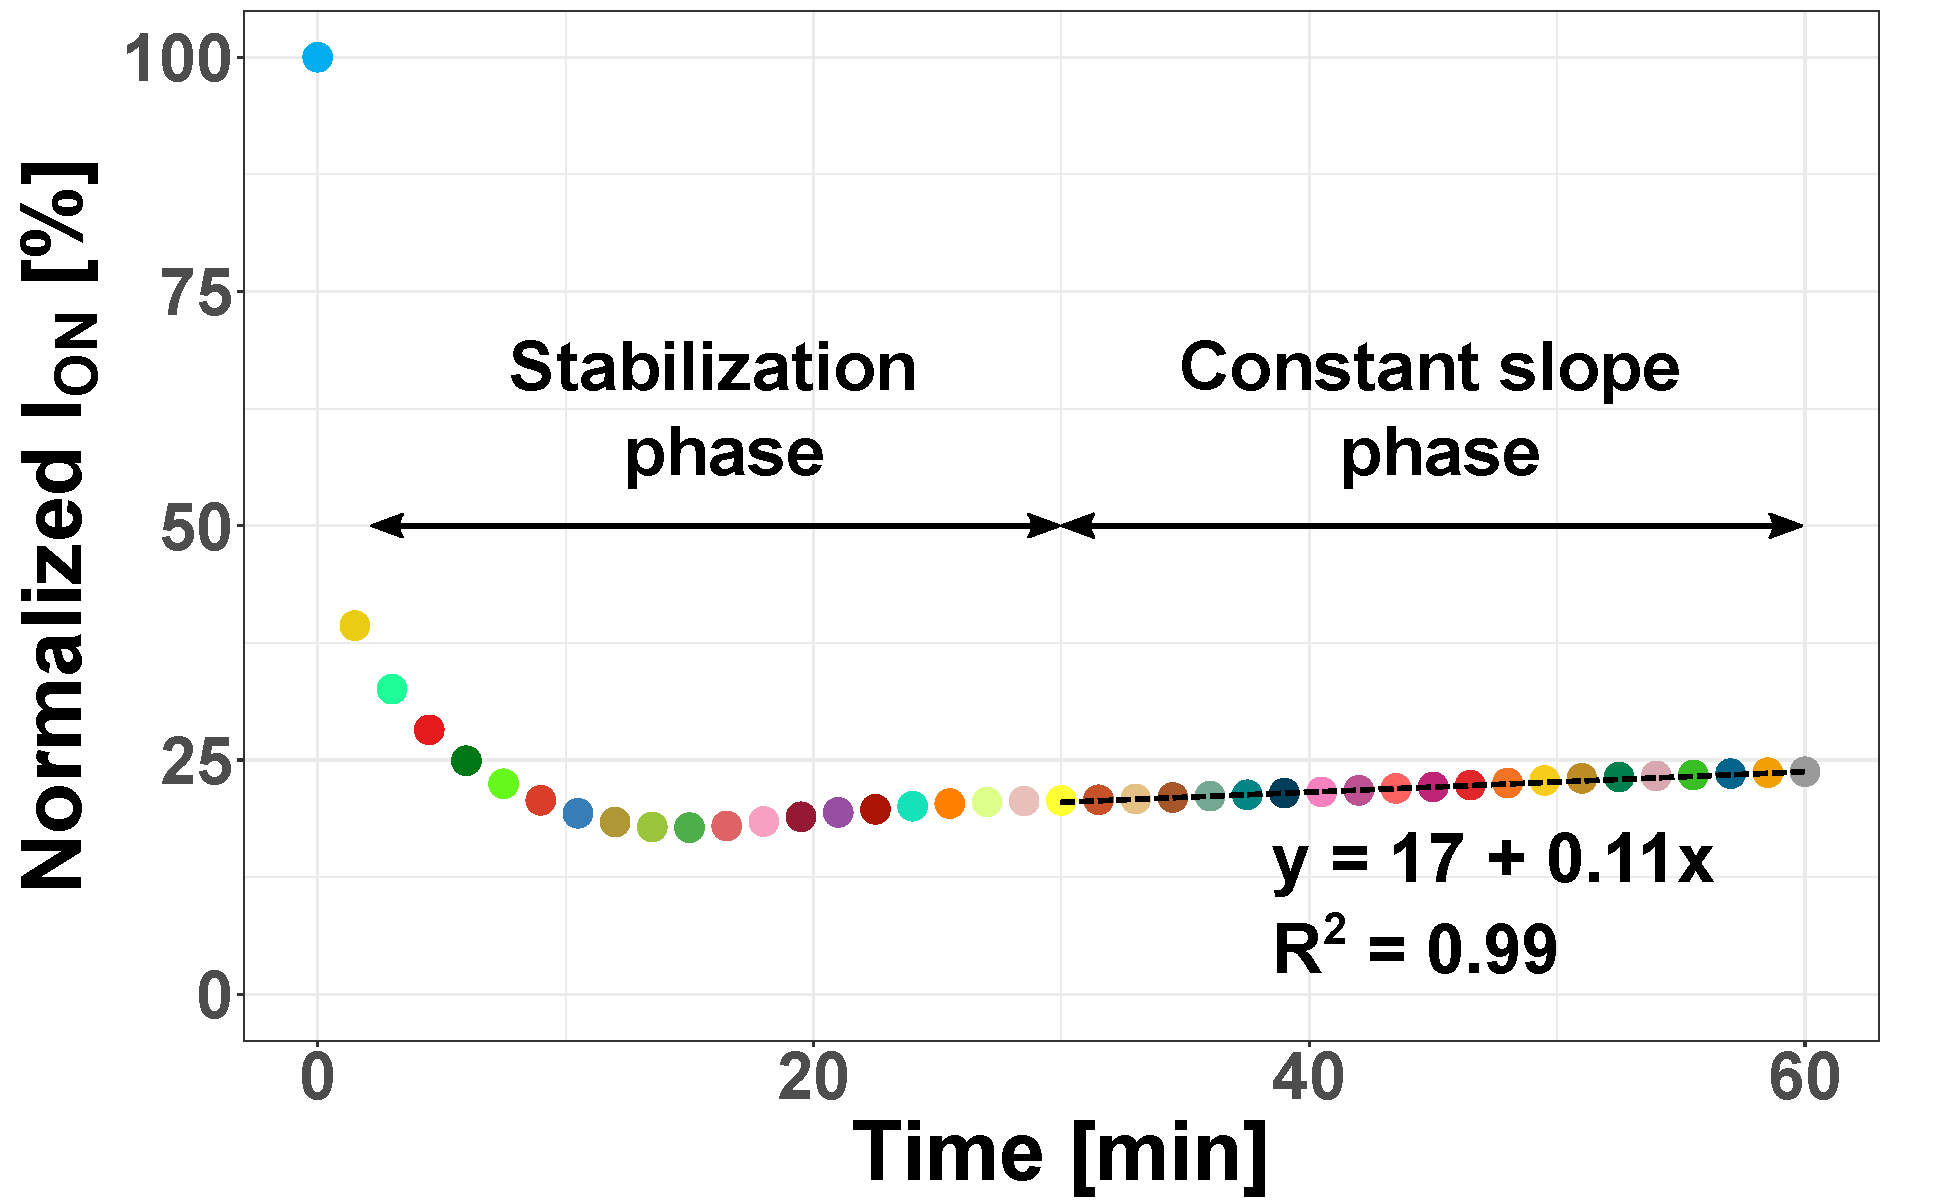
\includegraphics[width=0.45\textwidth]{figures/chapter3/EGFET/NormMem.pdf}%
        \label{fig:normMem}
    }
    \caption{\AT{I need the caption to a figure for a scientific paper: the figure contains two images depicting the first step of electrical characterization, \ie{} the transfer characteristics and the normalized \ion{}, basically repeating the same process as before. From these images we see a different trend than before, where the current now increases over time, implying a more stable performance.} \note{Initial step of electrical characterization, showing the transfer characteristics and the normalized \ion{}. These measurements follow the same procedure as previous analyses but reveal a different trend: the current now increases over time, indicating improved stability and more consistent device performance.}}
    \label{fig:Mem}
\end{figure}

\AT{Describe the transfer curves(Figure \ref{fig:transferMem}) of the devices with the encapsulated channel: we see a different trend from before: the first curve, the one collected 5 minutes after the start, is the one displaying the highest current, but after that it drops rapidly, only to start increasing again over time. Mention that the current is now one order of magnitude lower, if we look at it in absolute terms, but we basically don't care too much, because the signal is still good and we'd rather have a lower current that gives us more reliable results, rather than having a higher current that drops rapidly over time, until the device gets completely degraded and does not give a signal anymore. This current increase can be better observed looking at Figure \ref{fig:normMem}, which actually shows two distinct phases. From the start until approximately 30 minutes, the device is in the so-called \emph{stabilization phase}: during this phase, the EDLs still have to form, the ions are getting trapped in the membrane and an overall equilibrium still needs to be found. This can be seen from the fact that after the first point, the current decreaseas by more than half and keeps changing [for the lack of a better term, please find a more appropriate term to describe the fact that the \ion{} does not follow a linear trend at this point in the curve].
This equilibrium was found on average after \SI{33}{\min}, where the \ion{} becomes linear with respect to time. This is important in the case of EG-FETs used as transductors for sensors because this linear baseline can then be removed from the current measured during analyte detection and we can have more reliable measurements, to the point where we can plot a calibration curve and from this we are able to quantify the analyte in the samples. Overall, this shows a great improvement over state-of-the-art devices which reach this point after 60 minutes \cite{molazemhosseiniRapidly2021}. The second part of the plot is the so-called \emph{constant slope phase}, where the system is at equilibrium and the \ion{} displays a linear trend over time. In our analysis, we deemed a plot to be linear when $R^2>0.98$. On average it was found that our devices reached this linearity in \SI{33.8}{} $\pm$ \SI{12.9}{\min}, de facto halving the time of state-of-the-art devices.}

\note{The transfer curves of the devices with an encapsulated channel, shown in Figure \ref{fig:transferMem}, exhibit a markedly different trend compared to the unencapsulated counterparts. The first transfer curve, collected five minutes after the start, displays the highest current. However, this current rapidly decreases before gradually increasing again over time. In absolute terms, the current is now an order of magnitude lower than that of the unprotected devices. However, this reduction is not a major concern, as the signal remains well-defined. In fact, a lower but stable current is preferable to a higher current that degrades rapidly, ultimately leading to device failure and loss of signal integrity.
%
This current evolution is better visualized in Figure \ref{fig:normMem}, which highlights two distinct phases in the device behavior. The initial phase, lasting approximately 30 minutes, is referred to as the \emph{stabilization phase}. During this period, electrical double layers (EDLs) are still forming, ions are being trapped within the membrane, and the system is gradually moving toward equilibrium. This is evident from the fact that, after the first recorded point, the current drops by more than half and exhibits significant variability before settling [a more precise term to describe the non-linear behavior of \ion{} in this region]. 
%
On average, equilibrium is established after \SI{33}{\min}, at which point \ion{} follows a linear trend with respect to time. This stabilization is particularly relevant for electrolyte-gated field-effect transistors (EG-FETs) employed as transducers in sensor applications. A well-defined linear baseline can be subtracted from the measured current during analyte detection, improving measurement reliability. This enhancement allows for the construction of accurate calibration curves, ultimately enabling precise quantification of analytes in samples. Notably, our devices achieve stabilization significantly faster than state-of-the-art EG-FETs, which require approximately 60 minutes to reach the same point \cite{molazemhosseiniRapidly2021}.
%
Following the stabilization phase, the system enters the \emph{constant slope phase}, where \ion{} exhibits a consistent, linear trend over time. In our analysis, a dataset was considered linear when $R^2>0.98$. On average, the devices achieved this linearity in \SI{33.8}{} $\pm$ \SI{12.9}{\min}, effectively halving the stabilization time compared to previously reported devices. This significant improvement underscores the effectiveness of the encapsulation strategy in enhancing the stability and usability of EG-FET-based sensors.
}

\begin{figure}
    \centering
    \subfloat[\igs{} and \ids{}]{%
        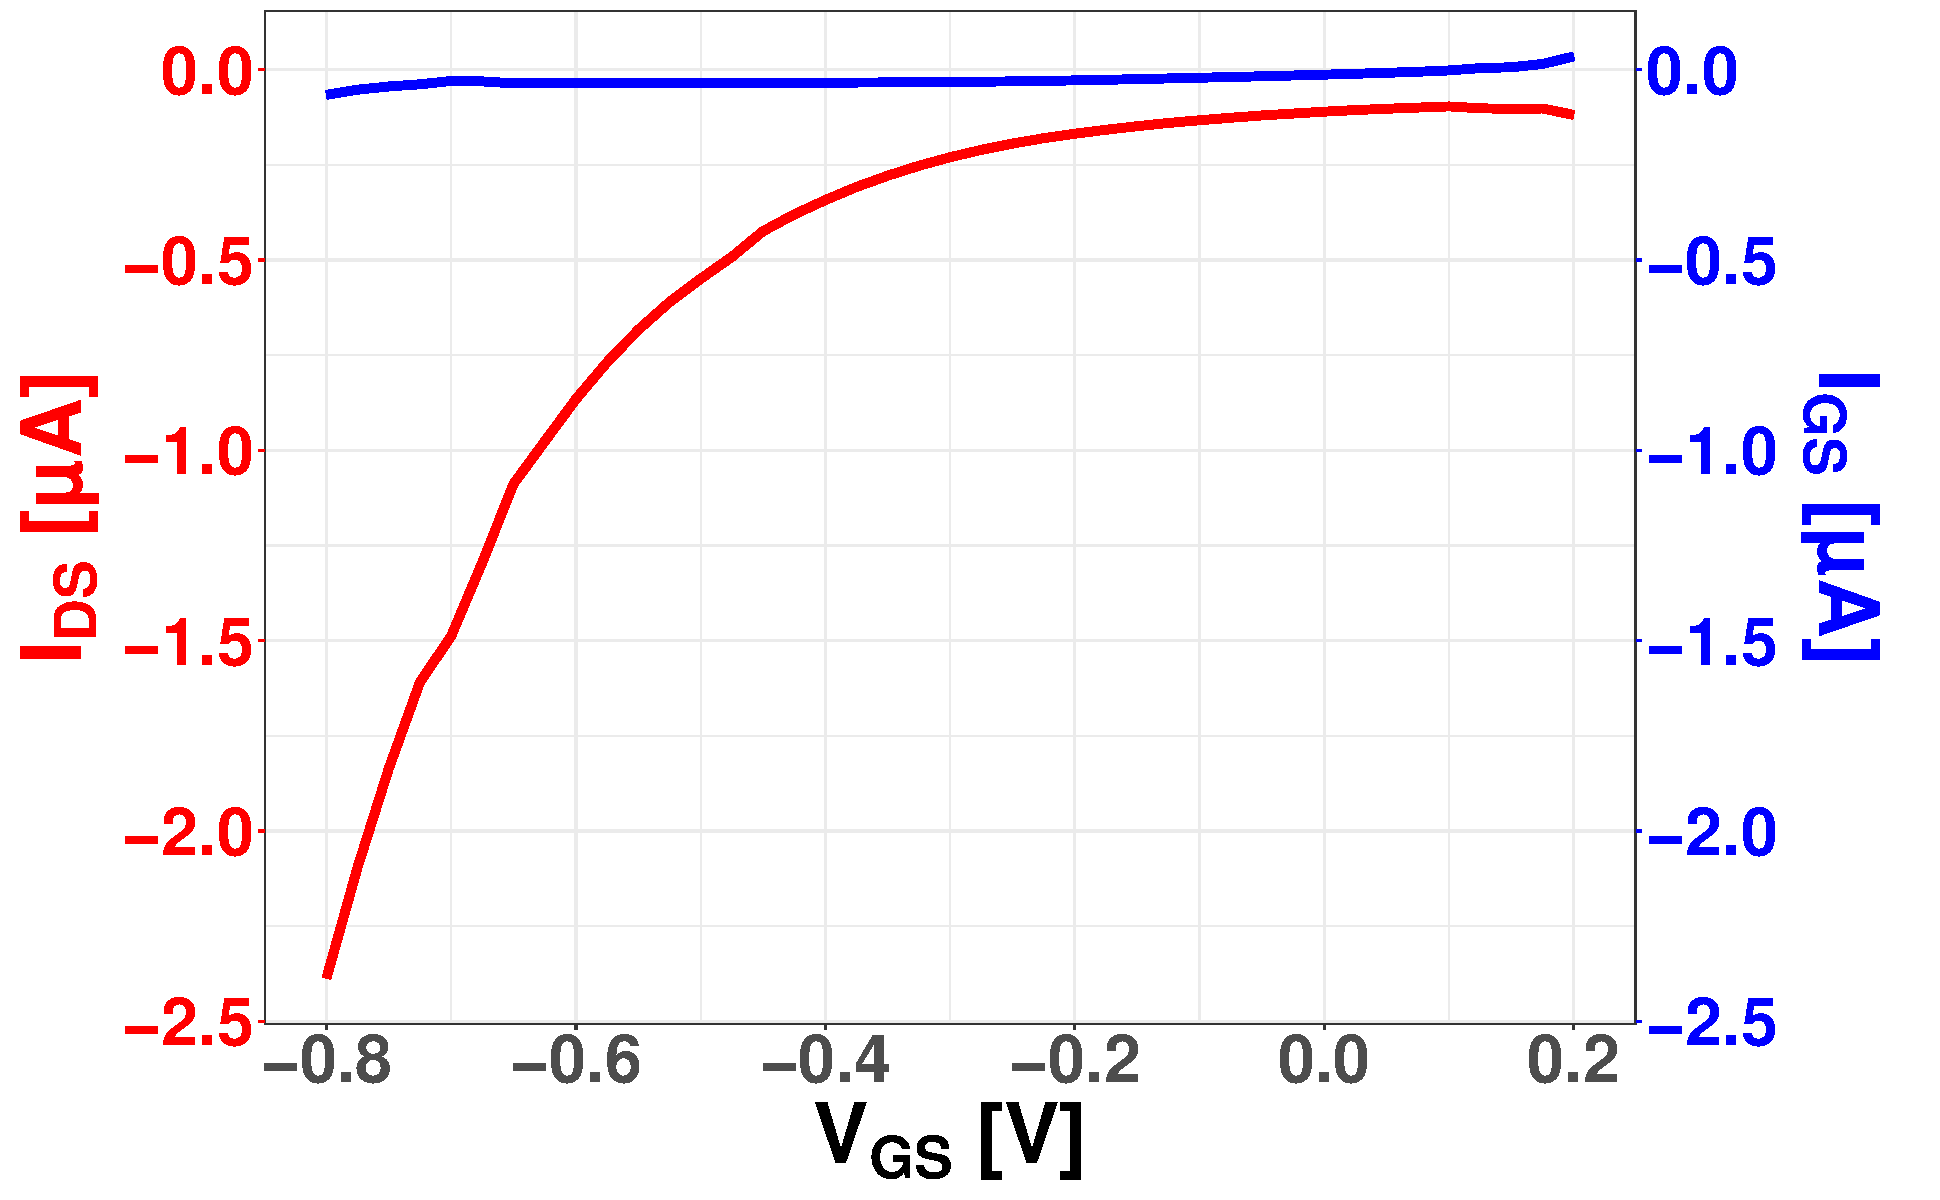
\includegraphics[width=0.45\textwidth]{figures/chapter3/EGFET/IdIgMem.pdf}%
        \label{fig:IdIgMemMem}
    }
    \quad
    \subfloat[Hysteresis]{%
        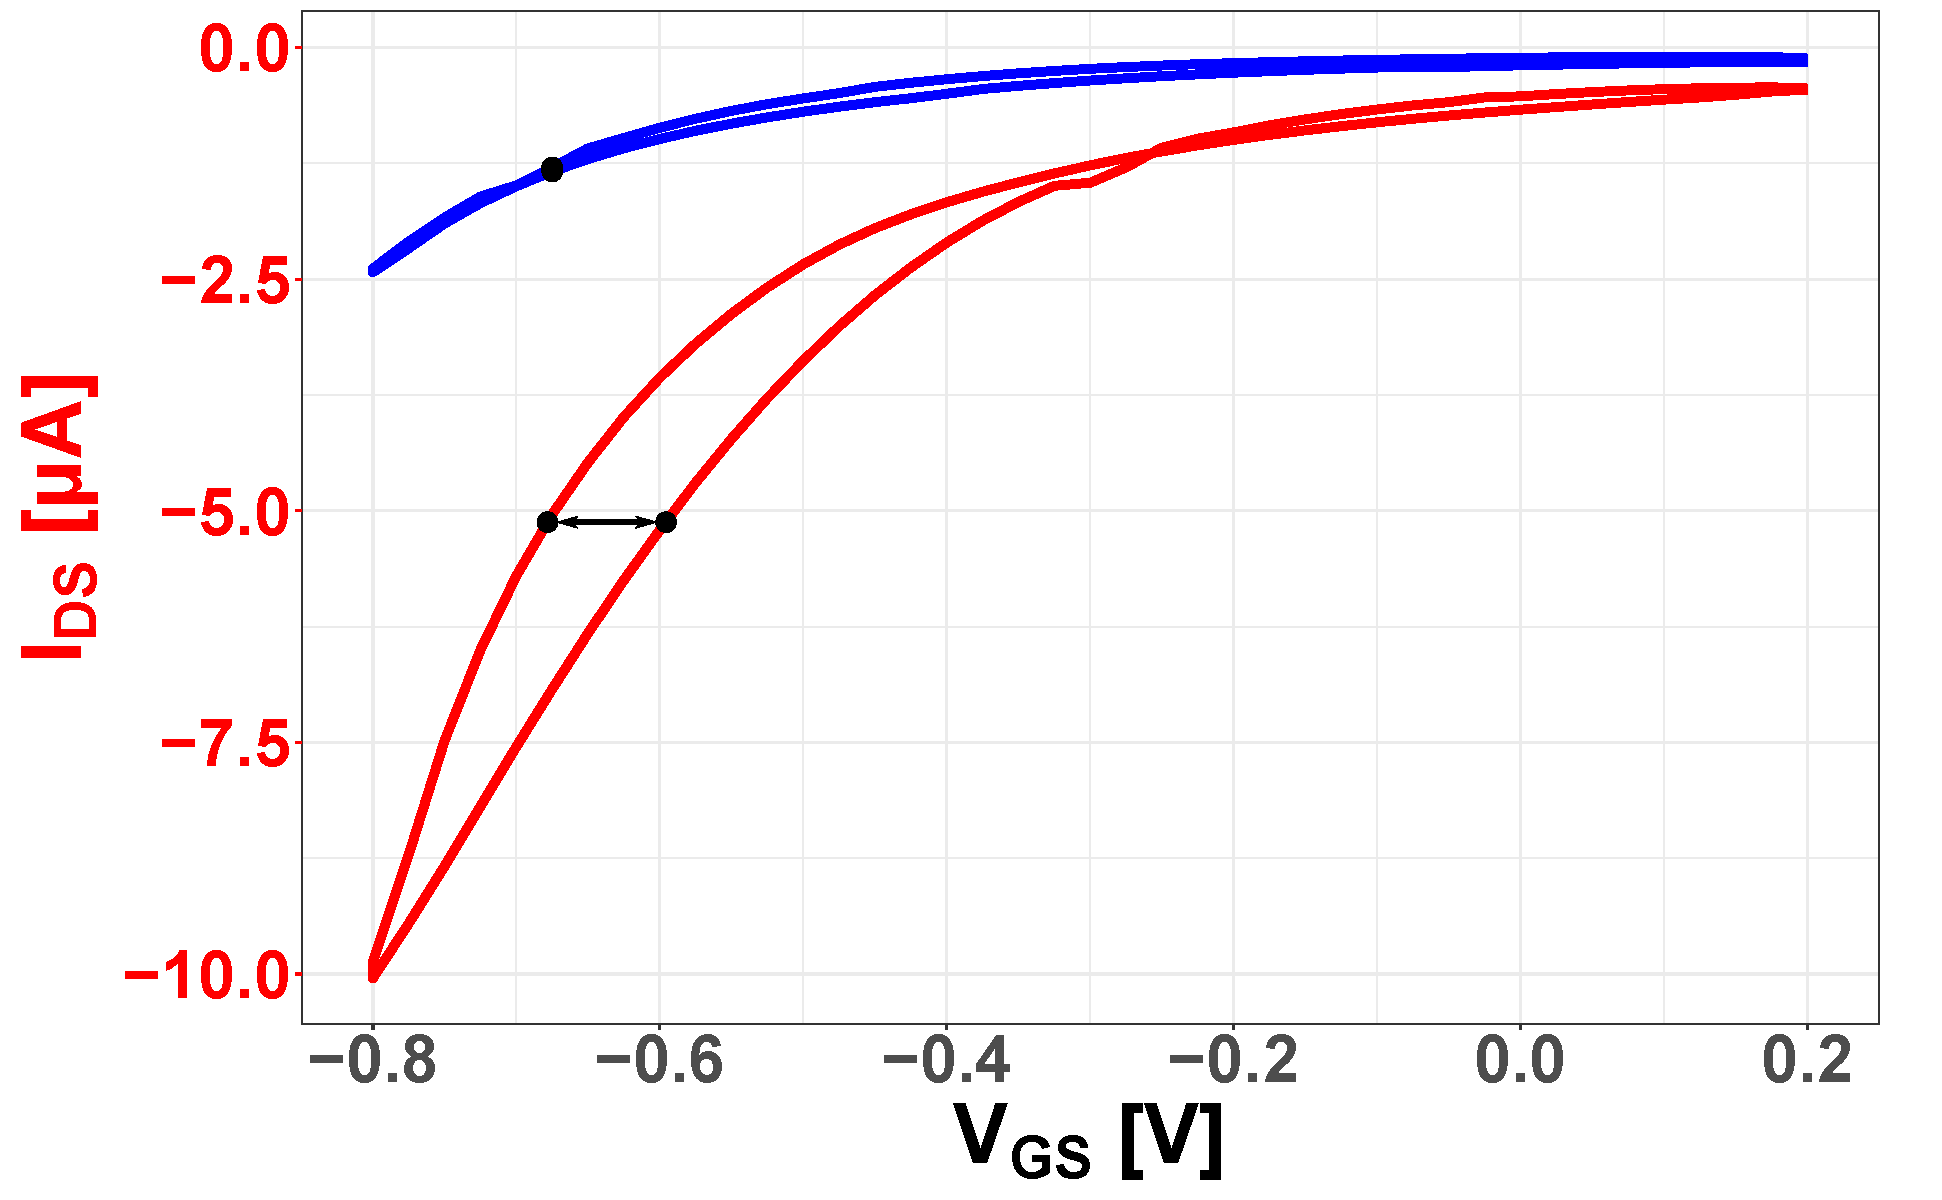
\includegraphics[width=0.45\textwidth]{figures/chapter3/EGFET/hysMem.pdf}%
        \label{fig:hysMem}
    }
    \caption{\AT{I need to write the caption to a figure for a scientific paper. Tie figure entails two images showing the \igs{} and \ids{} in one plot and the hysteresis in another, respectively. It is possible to see that also in this case, like in the case of bare channel, the gate current is orders of magnitude lower than the drain current, signifying low leakage [is it correct? What is the explanation? Why do we want low \igs{}?]. As for the hysteresis, we can see that it is lower for the devices with the membrane, even at the start of the experiment [what does this mean? why is a lower hysteresis good?]. It is noteworthy that also in this case, like before, the current decreases a lot from the first transfer recorded to the last, even though we have already seen that it starts increasing over time, contrary to what happens to the devices with the bare channel.} \note{Comparison of \igs{} and \ids{} (left) and hysteresis (right) for devices with a lipophilic membrane. As observed in the bare-channel case, the gate current remains orders of magnitude lower than the drain current, indicating low leakage and efficient gate control. A low \igs{} is desirable as it minimizes power dissipation and unwanted interference with the drain current. Regarding hysteresis, devices with the membrane exhibit reduced hysteresis even at the start of the experiment, suggesting improved charge stability and reduced trapping effects. Notably, although the current initially decreases significantly from the first to the last recorded transfer, it eventually begins to increase over time—contrary to the trend observed in bare-channel devices.}}
    \label{fig:parameters_Mem}
\end{figure}

\AT{Describe shortly Id Ig and hysteresis, highlight the differences with the bare devices say what's good and what's bad.}

\begin{figure}
    \centering
    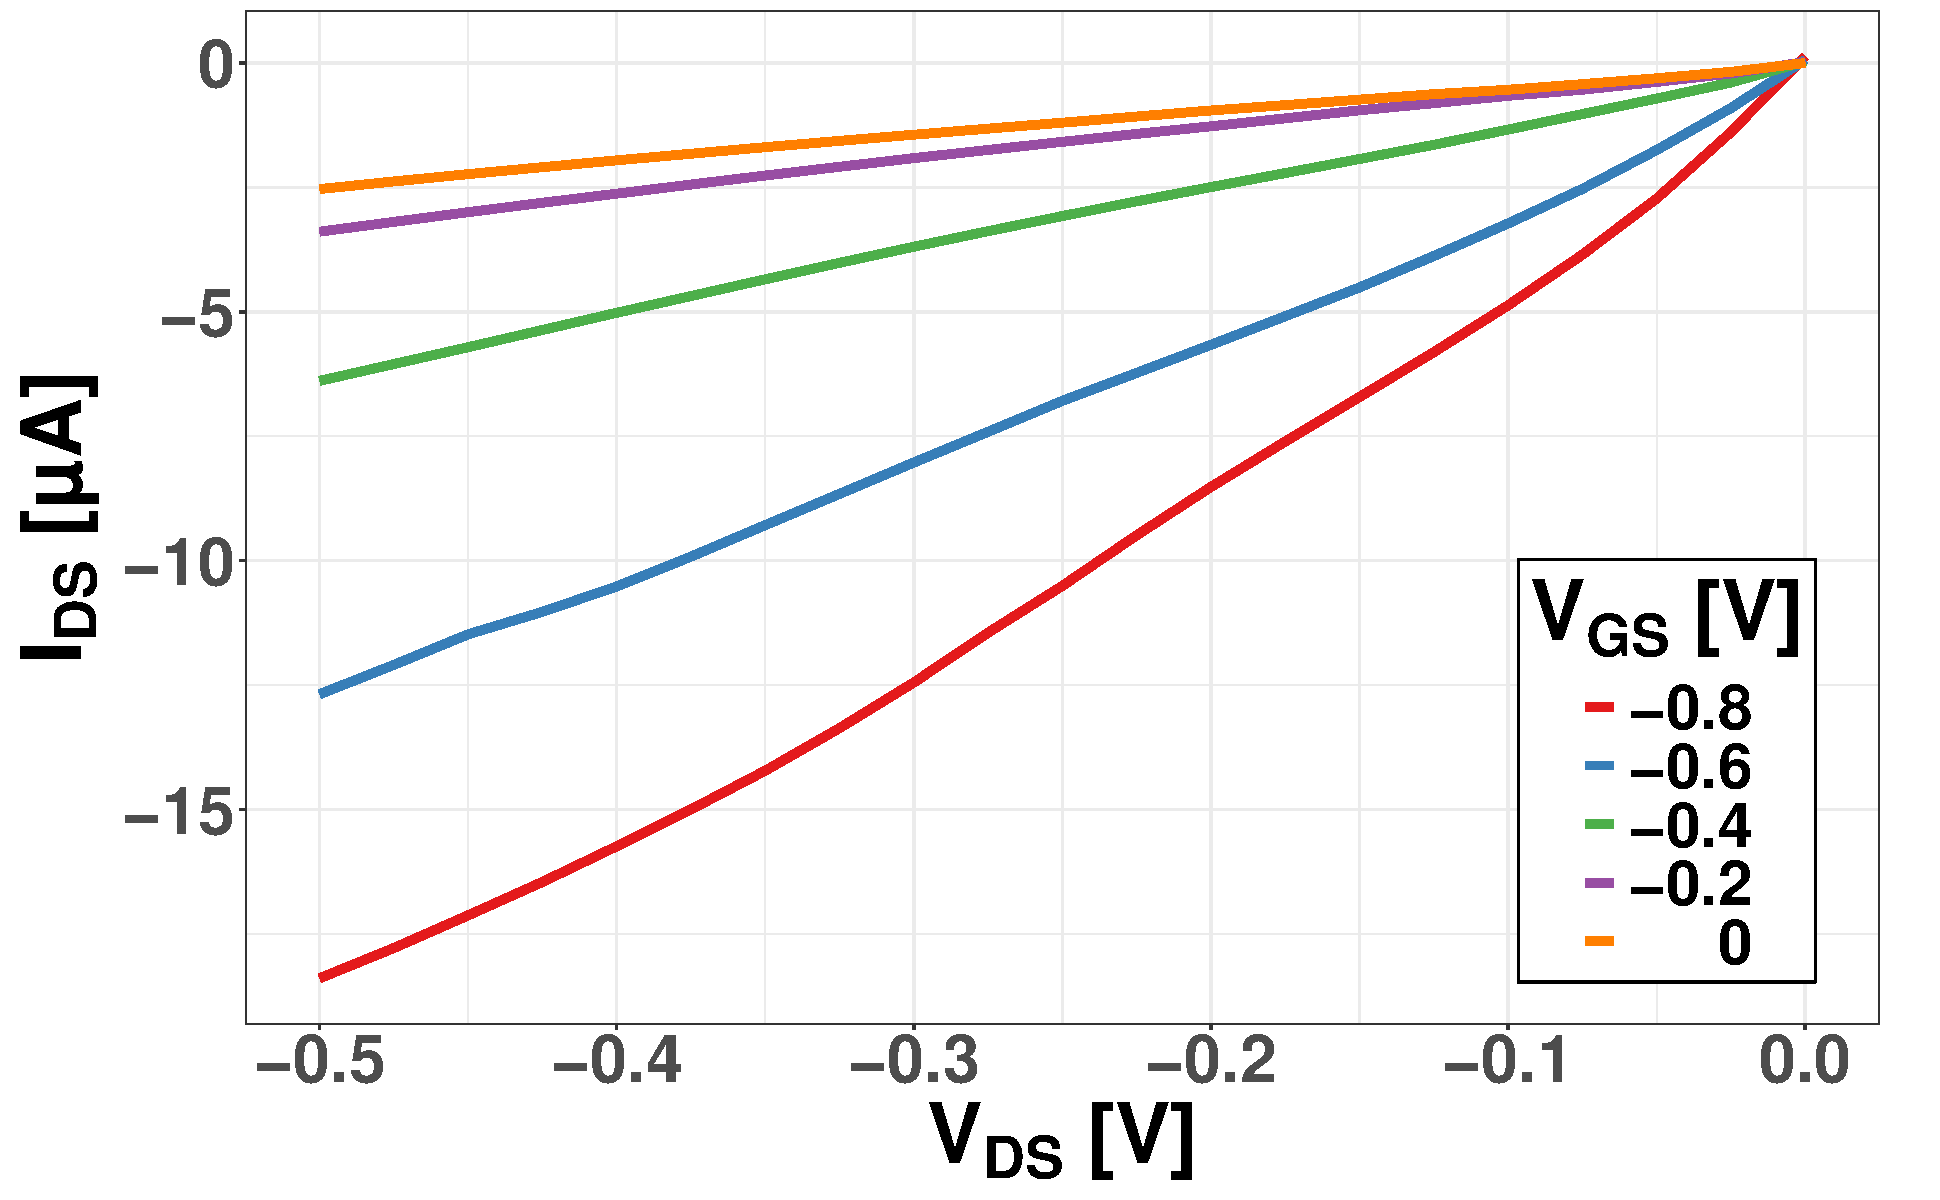
\includegraphics[width=0.45\textwidth]{figures/chapter3/EGFET/outputMem.pdf}
    \caption{\AT{I need to write the caption to a figure for a scientific paper. The figure displays the output characteristics for a device with encapsulated channel. The output curves displayed here are different than the ones in Figure \ref{fig:outputNoMem}, in the sense that here you can see that the devices are still very far from saturation, whereas before you could see the devices getting close to the saturation regime. [what does this say about the devices with the membrane? Is it good or is it bad? Is it neither? Is it just something that we observe? What can you infer from this?]} \note{Output characteristics of a device with an encapsulated channel. Compared to Figure \ref{fig:outputNoMem}, where devices approach the saturation regime, the output curves here indicate that the devices remain far from saturation. This suggests that the presence of the membrane affects charge transport and the formation of the accumulation layer, potentially modifying the gating efficiency. While this is not inherently good or bad, it is an important observation that may influence the device's operational mode and suitability for sensing applications. Further investigation is required to determine whether this behavior impacts sensitivity, response time, or overall performance.}}
    \label{fig:outputMem}
\end{figure}

\AT{Describe shortly the output characteristics and highlight differences with the devices without the membrane.}

\begin{figure}
    \centering
    \subfloat[4 hour measurement]{%
        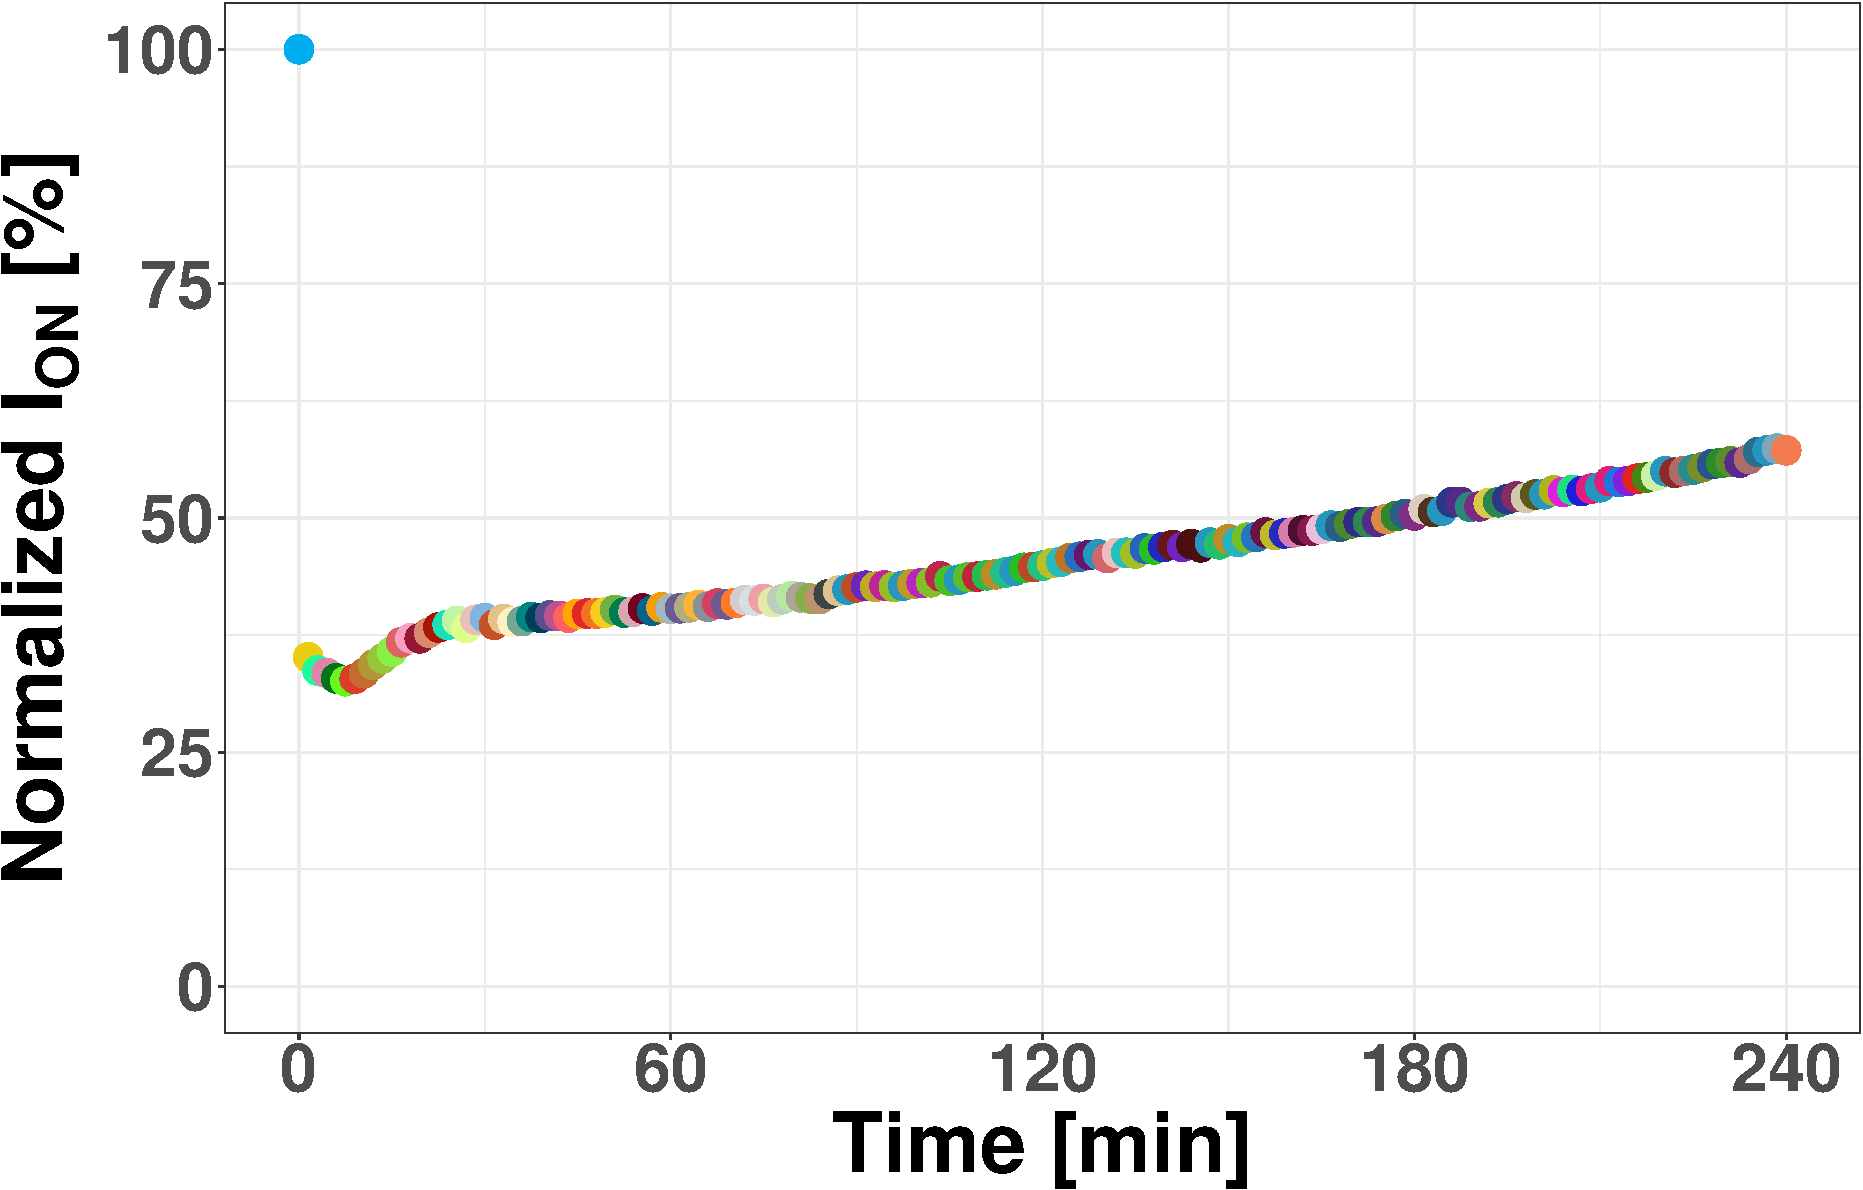
\includegraphics[width=0.45\textwidth]{figures/chapter3/EGFET/norm4h.pdf}%
        \label{fig:norm4h}
    }
    \quad
    \subfloat[12 hour measurement]{%
        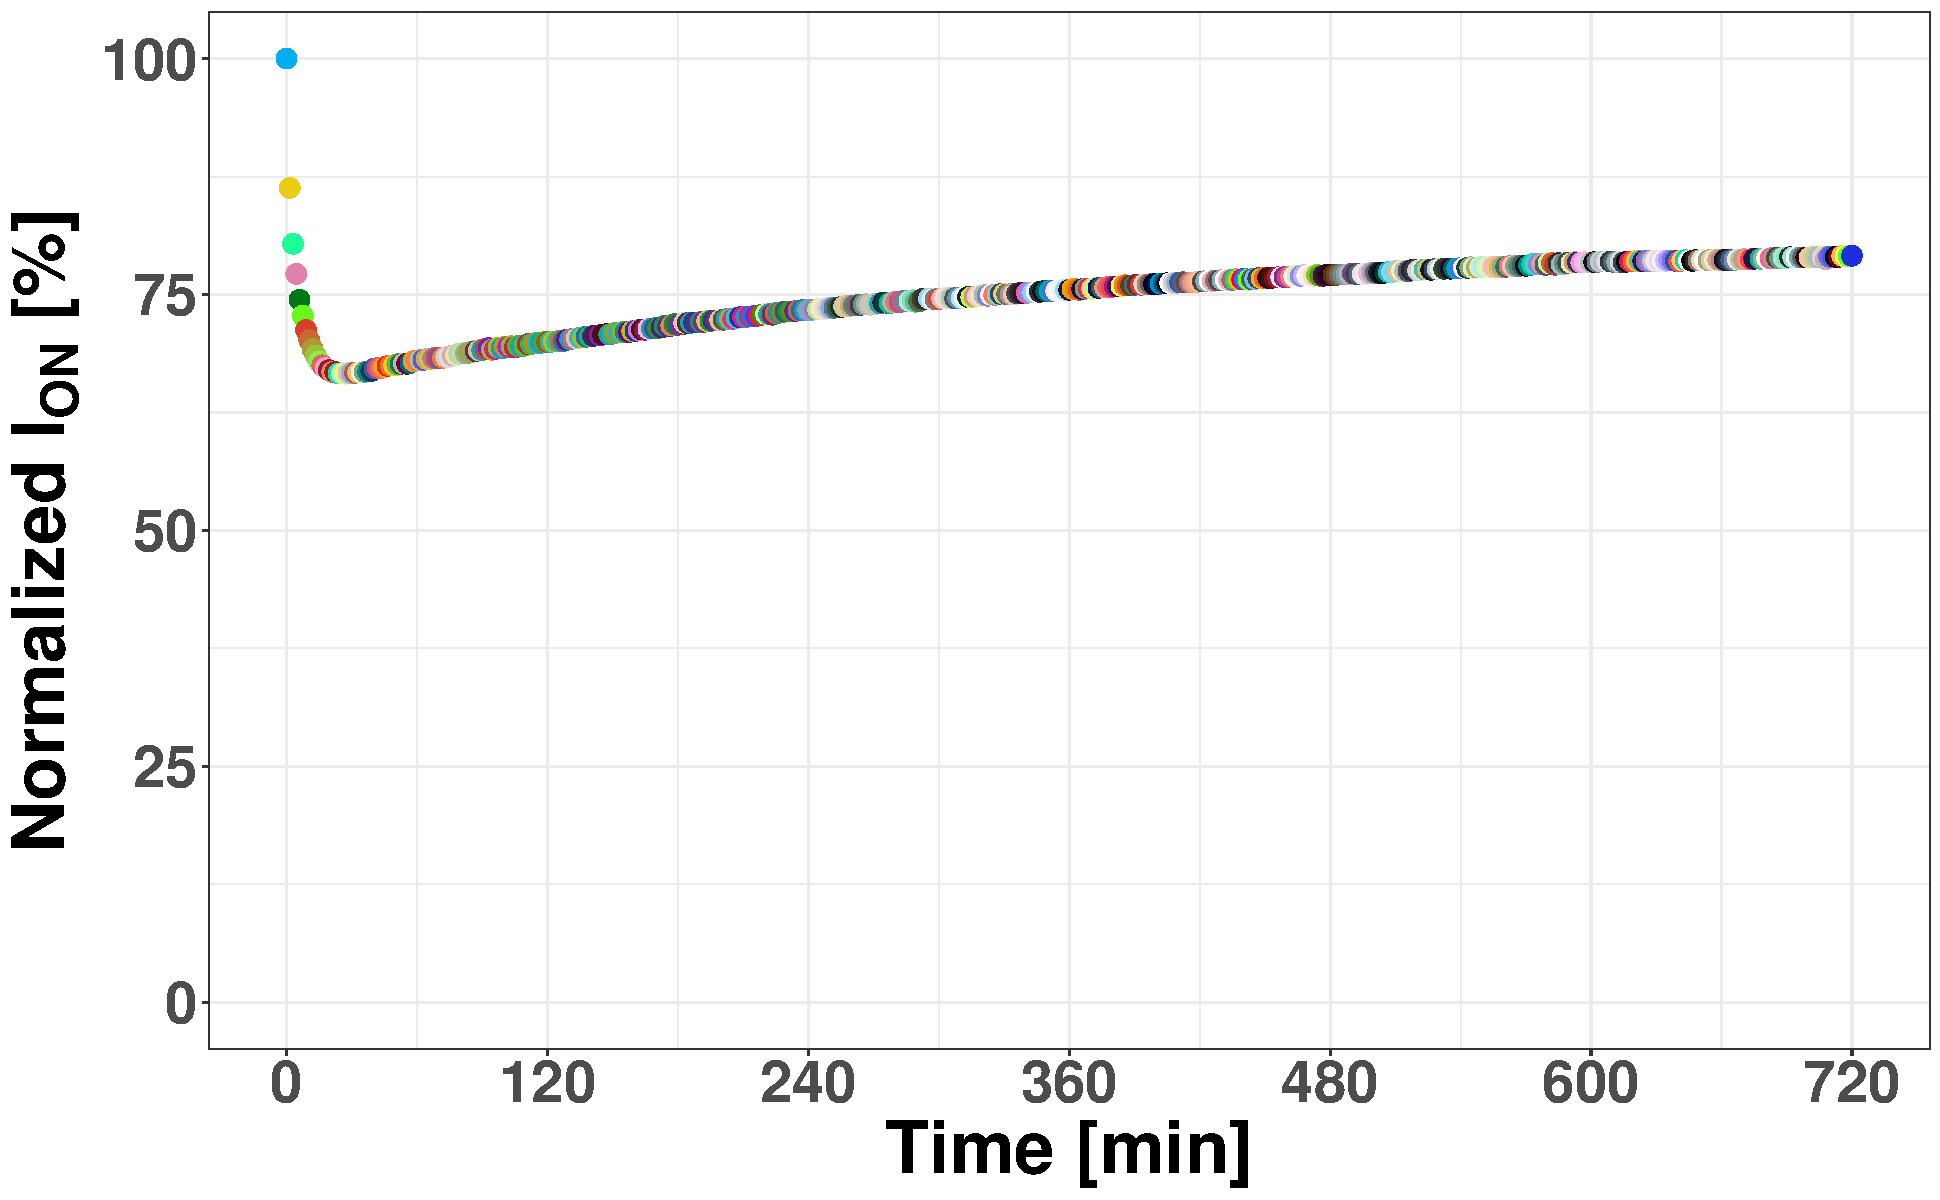
\includegraphics[width=0.45\textwidth]{figures/chapter3/EGFET/norm12h.pdf}%
        \label{fig:norm12h}
    }
    \caption{\AT{I need to write the caption to a figure for a scientific paper. The figure includes two images showing the normalized \ion{} for a prolonged time with respect to the standard experiment. Instead of collecting transfer characteristics for 60 minutes, the experiment went on for 4 hours (figure a) and for 12 hours (figure b). We can see that in both cases the current keeps increasing over time, indicating that even for prolonged times, the CNTs do not get degraded in the environment nor under electric stress.} \note{Normalized \ion{} over prolonged measurement periods. (a) Normalized \ion{} recorded over 4 hours and (b) over 12 hours, extending beyond the standard 60-minute experiment. In both cases, the current continues to increase over time, demonstrating that the CNTs remain stable without signs of degradation, even under extended environmental and electrical stress. This result confirms the long-term reliability of the devices, making them suitable for prolonged sensing applications.}}
    \label{fig:normLong}
\end{figure}

\AT{Describe how the devices with the membrane are highly stable even for prolonged times. In Figure \ref{fig:normLong} we can see the normalized \ion{} for 4 hours (\ref{fig:norm4h}) and for 12 hours (\ref{fig:norm12h}) and they both show that the current keeps increasing over time, maintaining the trend acquired before and thus the linearity needed for the use as sensor transducers. This is a great result because it means that our devices keep being reliable for long times, thus guaranteeing a good signal also when we use them as sensors.}

\note{The devices with the encapsulated channel demonstrate remarkable stability even over prolonged periods. Figure \ref{fig:normLong} presents the normalized \ion{} over extended measurement times, specifically for 4 hours (\ref{fig:norm4h}) and 12 hours (\ref{fig:norm12h}). Both datasets reveal a continued increase in current over time while maintaining the previously established trend. Importantly, the current follows a linear progression throughout these extended periods, ensuring the consistency required for EG-FETs to function effectively as sensor transducers.
%
This result is highly significant, as it confirms that the devices remain reliable over long durations, preserving signal integrity even during extended sensor operation. The ability to sustain a well-defined and predictable response over several hours enhances their practicality in real-world sensing applications, where prolonged stability is essential for accurate and reproducible analyte detection. By maintaining linearity in the signal over time, these devices offer a robust platform for sensor development, outperforming many conventional alternatives in terms of long-term usability and measurement consistency.
}

\begin{figure}
    \centering
    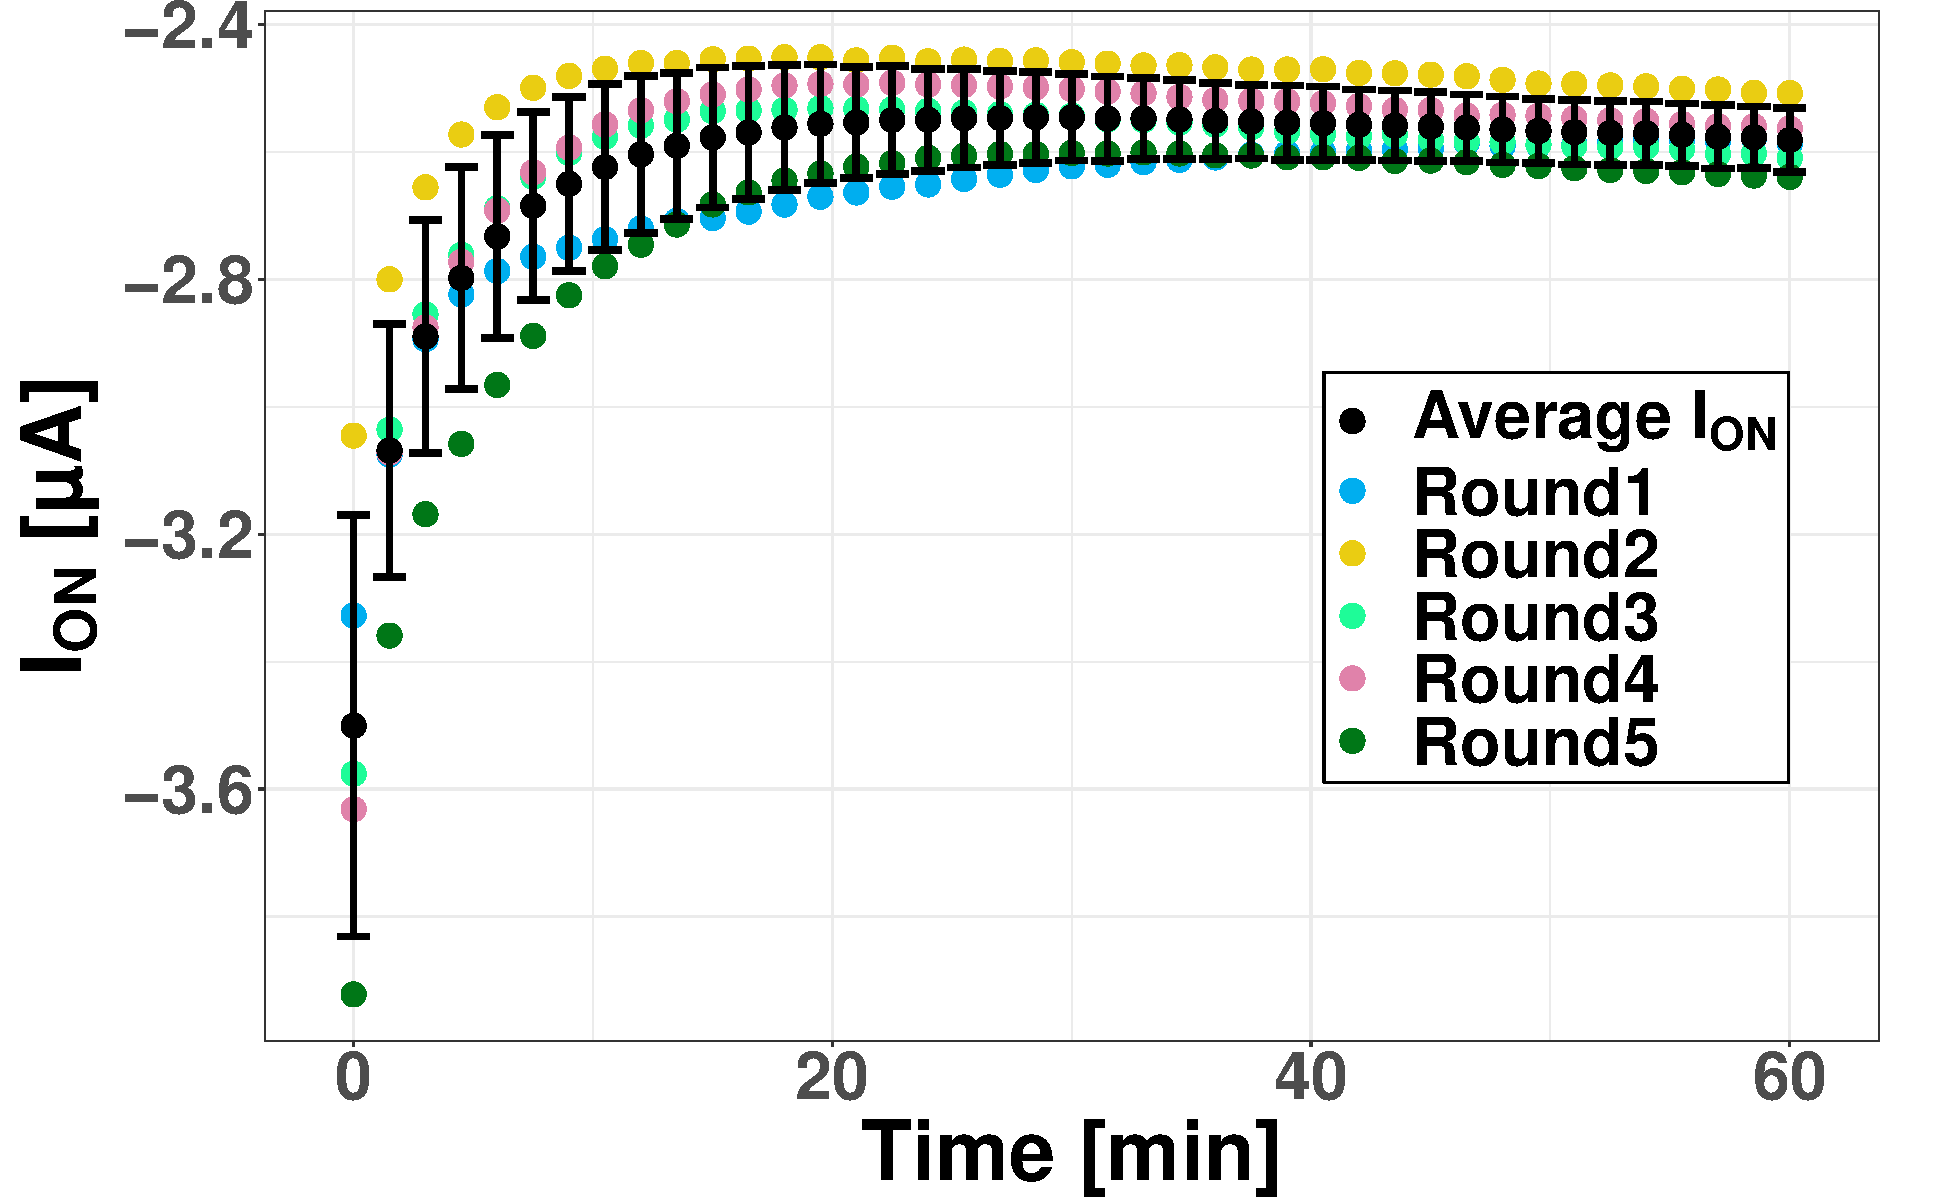
\includegraphics[width=0.45\textwidth]{figures/chapter3/EGFET/repMeas.pdf}
    \caption{\AT{I need to write the caption to a figure for a scientific paper: the figure shows the \ion{} for one device that underwent transfer collection 5 times; it is clear that the results are very reproducible from one cycle to the other; in fact, the variability among the five cycles amounts to 2.67\% after \SI{30}{\min} (the time necessary on average to reach an equilibrium), which is reduced to 1.93\% after \SI{60}{\min}} \note{Reproducibility of \ion{} over multiple measurement cycles. The figure shows the \ion{} for a single device undergoing five consecutive transfer characteristic collections. The results demonstrate high reproducibility, with variability among the five cycles amounting to just \SI{2.67}{\percent} after \SI{30}{\min} (the average time required to reach equilibrium), further reducing to \SI{1.93}{\percent} after \SI{60}{\min}. This consistency highlights the device's reliability for repeated use in sensing applications.}}
    \label{fig:repMeas}
\end{figure}

\AT{Describe the reproducibility of the measurements. We have proved that our devices, when they have the channel covered by a lipophilic membrane, they are very resistant to environmental and electrical stress. After the prolonged time stress test, we also tried to verify if they can resist to multiple uses (60 minutes, 40 cycles). The results obtained indicate that they can indeed be used multiple times (so far they have been tested 5 times), with very little variability among the different measurements. This result is particularly encouraging because it means that we can reuse the transducting component of the sensor, thus reducing the cost and the amount of trash that we generate.}

\note{The reproducibility of the measurements was also evaluated to assess the robustness of the devices under repeated use. Our results demonstrate that when the channel is covered by a lipophilic membrane, the devices exhibit strong resistance to both environmental and electrical stress. Following the prolonged time stress test, we further investigated their ability to withstand multiple measurement cycles. Specifically, each device was subjected to repeated use over \SI{60}{\min} sessions, spanning \num{40} cycles. 
%
The obtained results confirm that the devices maintain stable performance over multiple uses. Thus far, each device has been tested up to five times, displaying minimal variability between measurements. This outcome is particularly promising, as it indicates that the transducing component of the sensor can be reused without significant degradation. The ability to reuse the devices not only reduces operational costs but also minimizes electronic waste, making this approach more sustainable compared to single-use sensor platforms. These findings further support the long-term viability of the encapsulation strategy in improving the durability and practicality of EG-FET-based sensors.
}

\begin{figure}
    \centering
    \subfloat[Average On/Off ratio]{
        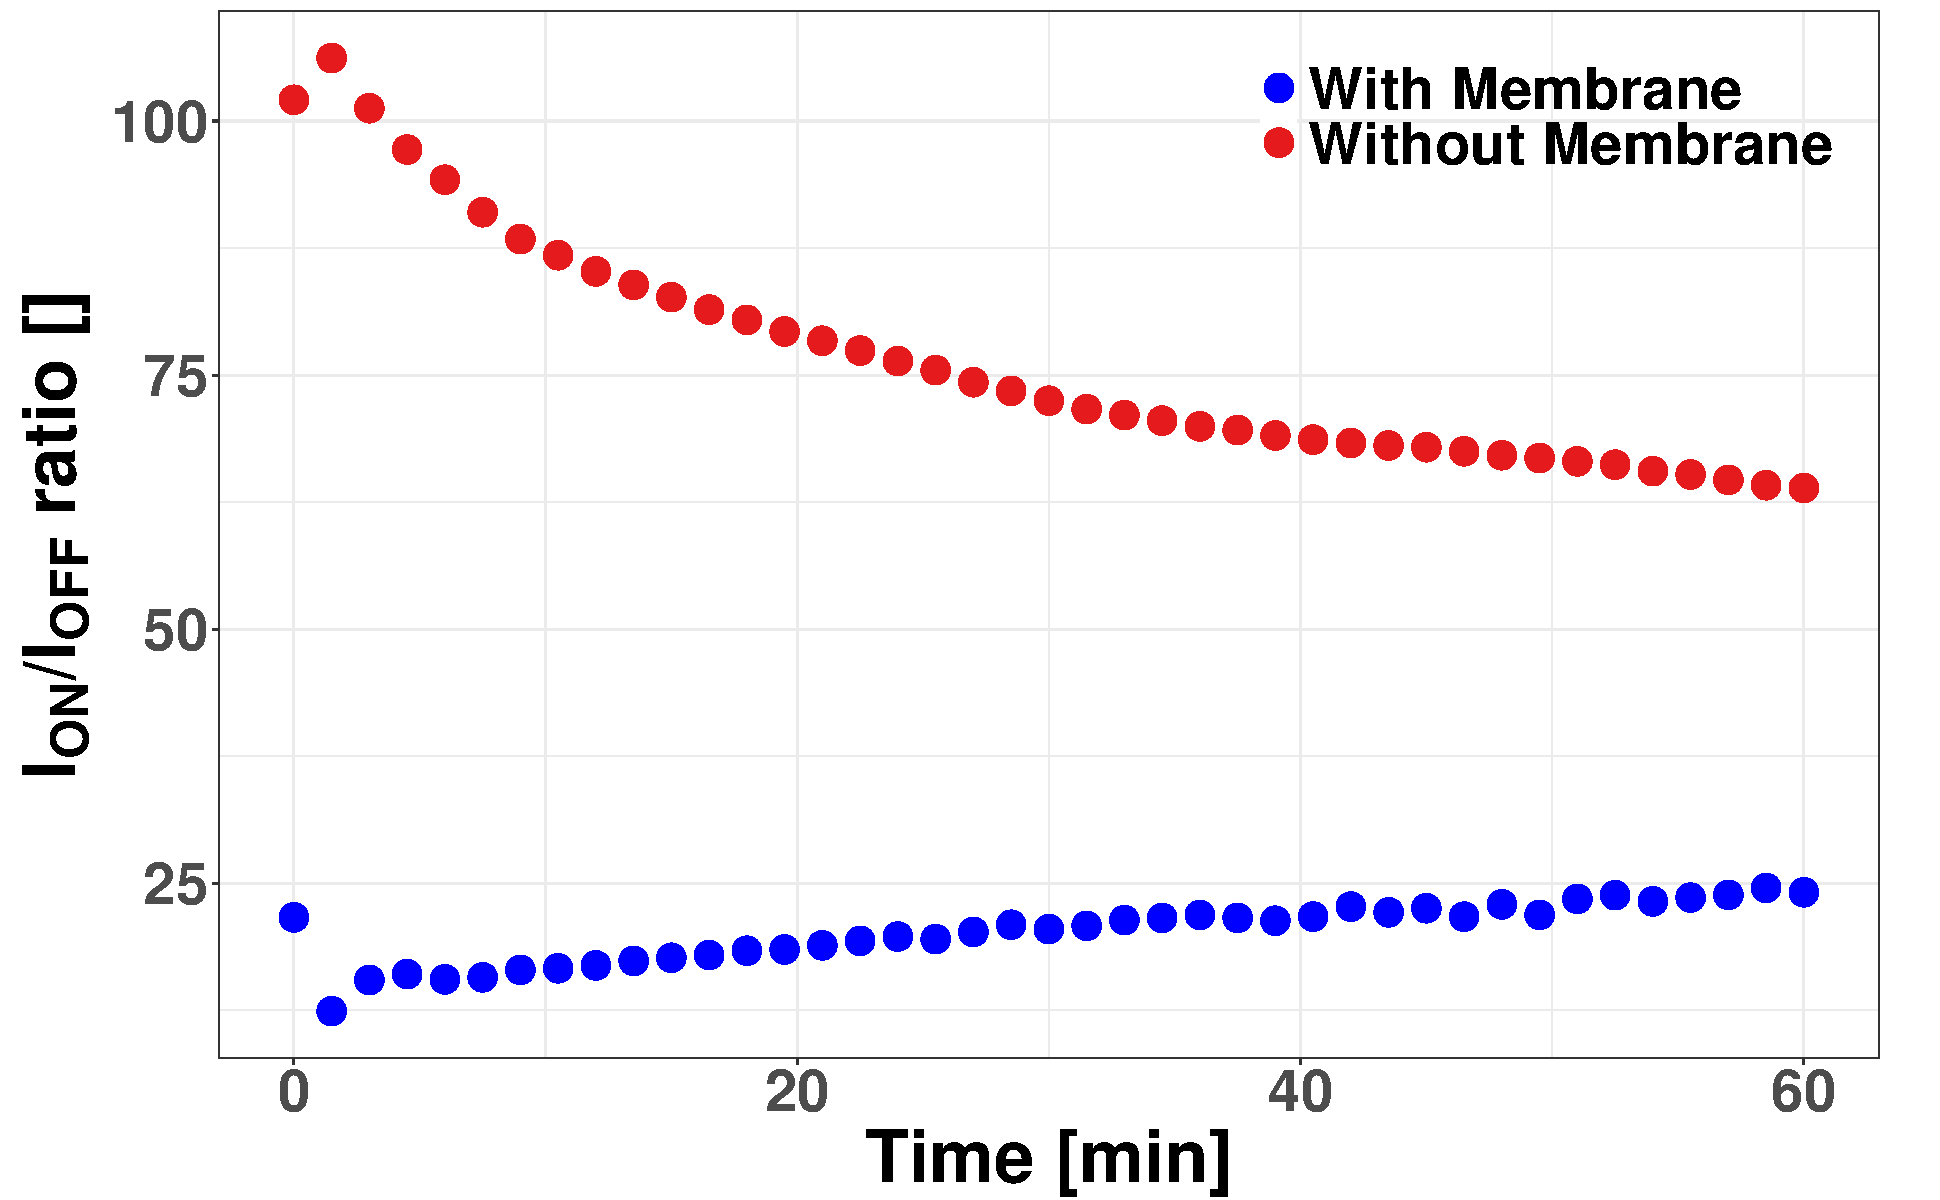
\includegraphics[width=0.45\textwidth]{figures/chapter3/EGFET/AvgOnOffRatio.pdf}
        \label{fig:avgOnOff}
    }
    \hfill
    \subfloat[Average threshold voltage]{
        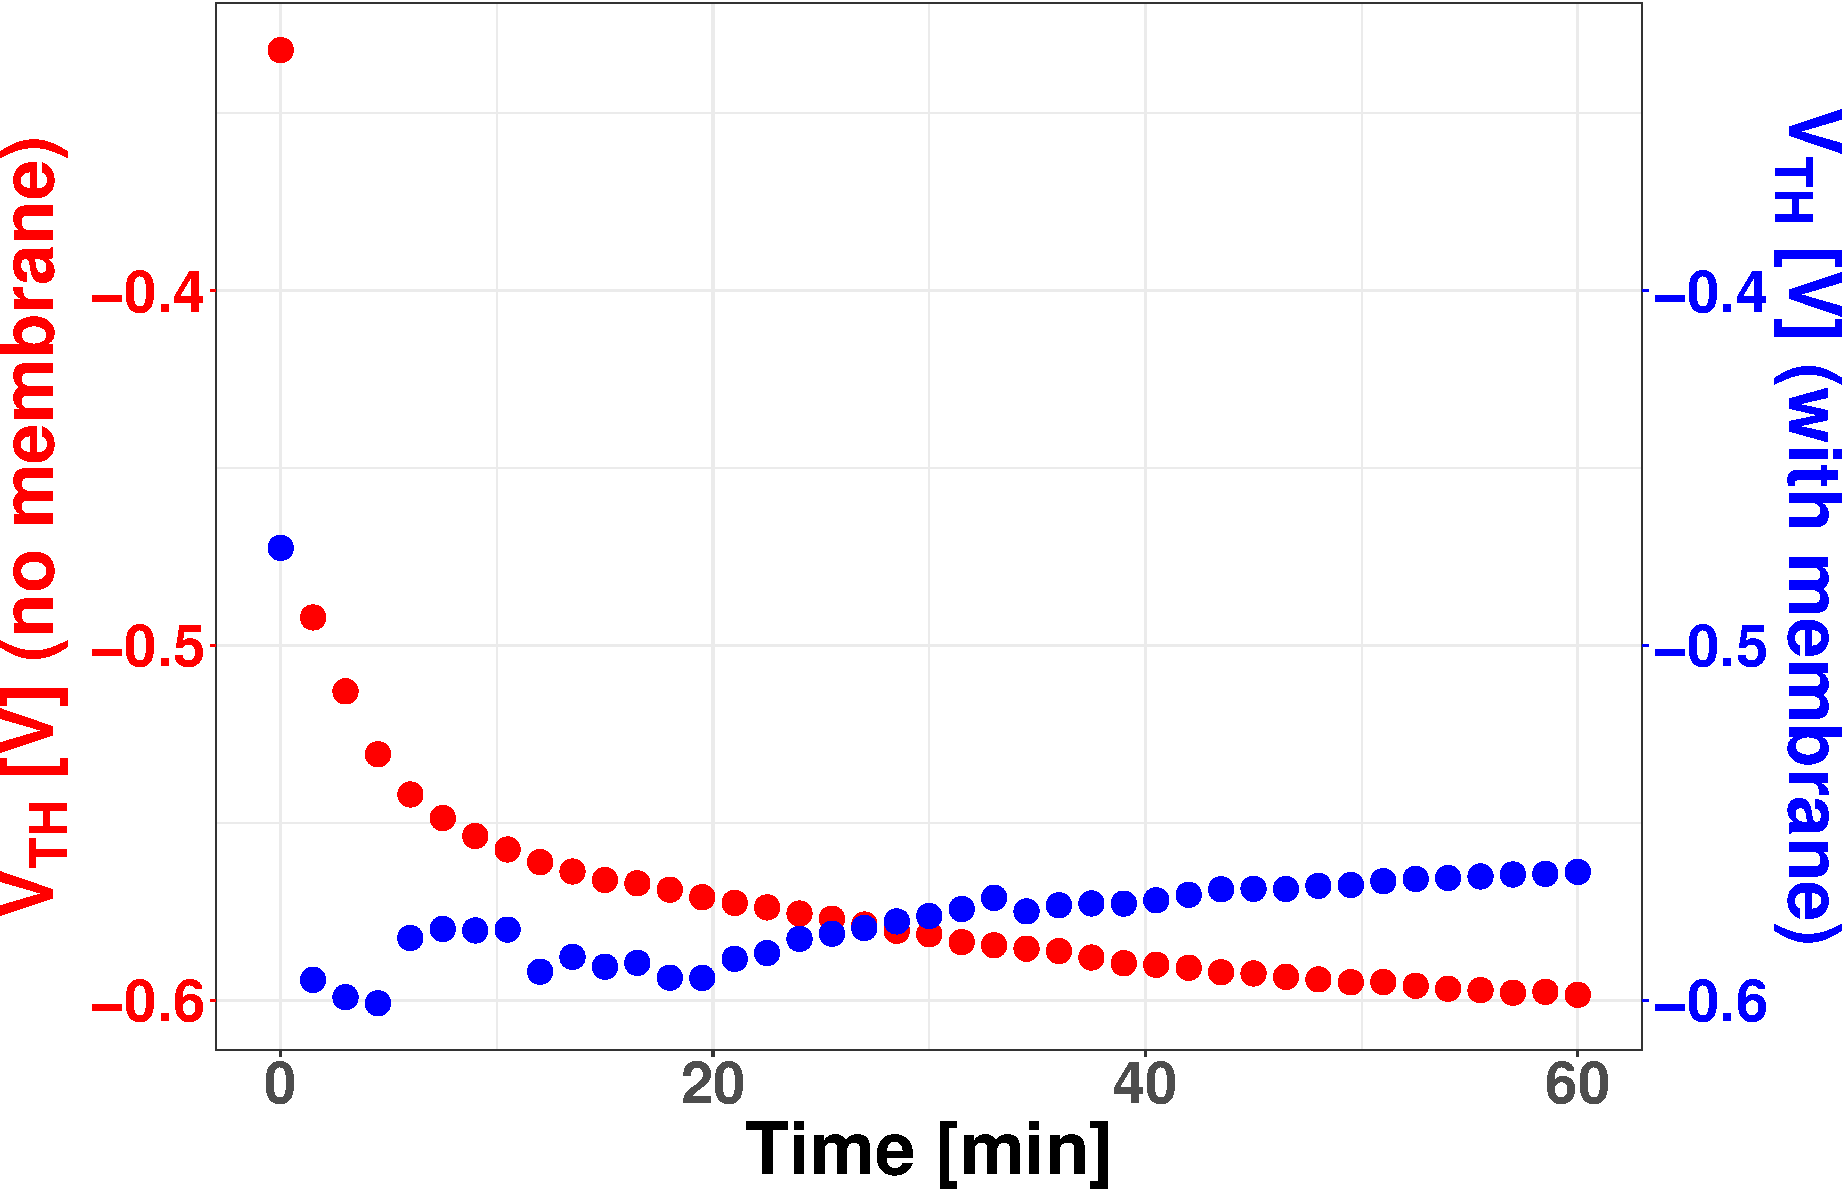
\includegraphics[width=0.45\textwidth]{figures/chapter3/EGFET/AvgVth.pdf}
        \label{fig:avgVth}
    }
    \caption{Comparison of average electrical parameters for device without the membrane (n = 3) and devices with the membrane (n = 6): (a) On/Off ratio and (b) threshold voltage.}
    \label{fig:avgParamsCfr}
\end{figure}

\AT{In Figure \ref{fig:avgParamsCfr} we show a couple more parameters that are indicative of the performance of the devices. In Figure \ref{fig:avgOnOff} I have to describe, analyze and comapre the trend of the on/off ratio of devices without and with the lipophilic membrane. The bare devices show a decrease of the ratio from nearly 100 to a stabilized level around 60, representing a pretty big drop, and indicating a deterioration in device performance. In contrast, devices with membrane-protected CNTs show a continuous linear increase over time; after a first drastic drop, from 17.63 to 9, the ION/IOFF continues to increase to 24.51, leading to an overall improvement in performance over time.
In Figure \ref{fig:avgVth}, we observe the average \vth{} for devices without a
membrane and devices with the membrane in red
and blue, respectively. From this plot we can clearly see that
this parameter keeps increasing in modulus for membrane-less
devices, meaning that more energy is needed to turn on the device, leading to increased energy expenditure [is this correct? How would you explain it better? does the vth have any other meaning?].}

\note{Figure \ref{fig:avgParamsCfr} presents additional key parameters indicative of device performance. In particular, Figure \ref{fig:avgOnOff} compares the evolution of the ON/OFF ratio (\ratio{}) for devices without and with the lipophilic membrane. The bare devices exhibit a substantial decline in the ON/OFF ratio, dropping from nearly 100 to a stabilized level of approximately \num{60}. This significant reduction indicates a deterioration in device performance over time, likely due to environmental degradation and charge trapping effects.  
%
In contrast, devices with membrane-protected CNTs display a markedly different trend. After an initial drop from \num{17.63} to \num{9}, the \ratio{} exhibits a continuous linear increase, eventually reaching 24.51. This steady improvement over time suggests that the encapsulated devices experience progressive stabilization, leading to enhanced overall performance. The membrane effectively mitigates environmental effects, reducing the rate of CNT degradation and promoting more reliable long-term operation.  
%
Figure \ref{fig:avgVth} illustrates the average threshold voltage (\vth{}) for both unprotected (red) and membrane-protected (blue) devices. A clear distinction emerges between the two cases: for the unprotected devices, \vth{} continuously increases in modulus, meaning that the device requires a higher gate voltage to reach the conductive state. This shift suggests an increase in charge trapping or oxidation-related effects, ultimately leading to greater energy expenditure during operation.  
%
Conversely, the \vth{} of membrane-protected devices remains more stable over time, further supporting the hypothesis that the encapsulation minimizes external influences on the CNT network. Maintaining a stable \vth{} is particularly important for sensor applications, as it ensures predictable device behavior, improved reproducibility, and lower power consumption over extended use. These findings further highlight the benefits of incorporating a protective membrane to enhance the stability and longevity of EG-FETs.  
}


\AT{Insert and discuss figures in Padova!}